%! TeX program = xelatex 
%! TeX root = main.tex

% Formato de la hoja
\documentclass[letterpaper, 12pt, oneside]{book} % carta, letra: 12
\renewcommand{\baselinestretch}{1.5} % Interlineado general
\usepackage[margin=2.5cm, top=4cm, left=4cm]{geometry}

% Fuente 
\usepackage{fontspec}
\usepackage{fontawesome5}
\setmainfont{Arial}
% \usepackage{helvet}
% \renewcommand{\familydefault}{\sfdefault}
% \usepackage[T1]{fontenc}

% Para insertar Imágenes
\usepackage{graphicx}
\graphicspath{{./figuras}}
% \DeclareGraphicsExtensions{.png,.pdf}

% Paquetes
\usepackage[english, spanish, es-tabla]{babel} % configuración en español
\usepackage{wrapfig} % envolver imágenes alrededor de texto (logo utem)
\usepackage{parskip} % formato de texto con salto de párrafo
\usepackage{tabularx, booktabs} % mejores tablas
\usepackage{hyperref} % insertar enlaces dentro del documento
\usepackage{xurl} % insertar url's directamente
\usepackage{verbatim} % para usar texto monoespaciado como código
\usepackage{listings} % para formatear texto como código
\usepackage{setspace} % personalizaciones de espaciado
\usepackage{enumitem} % para personalizar los entornos enumerate, itemize.
\usepackage[dvipsnames, table]{xcolor} % definir colores personalizados
\usepackage[labelfont=bf,justification=raggedright,singlelinecheck=false]{caption} % personalizar entornos de citas
\usepackage{fancyhdr} % personalizar header/footer
\usepackage{lastpage} % personalizar numeración de páginas/titulos
\usepackage{titlesec} % personalizar títulos
\usepackage{float} % opciones de elementos flotantes (figuras)
\usepackage[bottom]{footmisc} % personalizar pié de página
\usepackage{rotating} % rotar figuras
\usepackage[export]{adjustbox}
\usepackage{placeins}
\usepackage{tikz}
\usepackage[titles]{tocloft}

\usepackage[nonumberlist, acronym]{glossaries}
\newglossary[glg]{negocio}{gls}{glo}{Glosario del Negocio}
\newglossary[glg]{tech}{tls}{tlo}{Glosario Técnico}

\makeglossaries

\newglossaryentry{corte}{
    type=negocio,
    name={Corte},
    description={Proceso interno de confección de uniformes de la entidad que provee los uniformes corporativos (proveedor)}
}
\newglossaryentry{segmento}{
    type=negocio,
    name={Segmento},
    description={Conjunto de prendas perteneciente a un área de desempeño en la empresa, por ejemplo vigilante, secretaria, etc. Masculinos y femeninos forman parte de segmentos distintos. Generalmente un proveedor se encarga de la confección de un solo segmento}
}
\newglossaryentry{envioacorte}{
    type=negocio,
    name={Envío a Corte},
    description={Solicitud que realiza el administrador de la institución que necesita uniformes al proveedor para indicar cuántos uniformes deben confeccionarse, basándose en la cantidad de funcionarios registrados con sus tallas ingresadas durante la temporada. En una misma temporada pueden generarse varias solicitudes. Dependiendo de la cantidad de funcionarios con tallas ingresadas, el administrador puede decidir cuándo enviar a corte y a cuántos funcionarios enviar}
}
\newglossaryentry{temporada}{
    type=negocio,
    name={Temporada},
    description={Período de tiempo definido por el administrador para organizar la solicitud y entrega de uniformes, por ejemplo una temporada de invierno y otra de verano, cada una con sus propios plazos y requerimientos}
}
\newglossaryentry{curvadetalla}{
    type=negocio,
    name={Curva de talla},
    description={Distribución de tallas por cada prenda}
}
\newglossaryentry{guiadedespacho}{
    type=negocio,
    name={Guía de despacho},
    description={Documento tributario electrónico destinado a acreditar el traslado de los uniformes desde la fábrica del proveedor a la respectiva sucursal definida}
}
\newglossaryentry{autenticacion}{
    type=tech,
    name={Autenticación},
    description={Proceso mediante el cual un sistema verifica la identidad de un usuario antes de permitir su acceso}
}
\newglossaryentry{autorizacion}{
    type=tech,
    name={Autorización},
    description={Proceso que determina los permisos y privilegios que tiene un usuario dentro del sistema}
}
\newglossaryentry{backend}{
    type=tech,
    name={Back-end},
    description={Conjunto de servicios, lógica de negocio y operaciones del sistema ejecutadas en el servidor}
}

\newglossaryentry{basededatosrelacional}{
    type=tech,
    name={Base de datos relacional},
    description={Modelo de almacenamiento que organiza información en tablas relacionadas mediante claves}
}

\newglossaryentry{bigballofmud}{
    type=tech,
    name={Big Ball of Mud},
    description={Antipatrón que describe sistemas sin arquitectura clara, con alto acoplamiento y baja mantenibilidad}
}

\newglossaryentry{cloudcomputing}{
    type=tech,
    name={Cloud Computing},
    description={Modelo de provisión de servicios computacionales a través de Internet bajo demanda}
}

\newglossaryentry{contenedor}{
    type=tech,
    name={Contenedor},
    description={Unidad portátil que empaqueta una aplicación junto con sus dependencias para ejecutarse de forma consistente en distintos entornos}
}

\newglossaryentry{desacoplamiento}{
    type=tech,
    name={Desacoplamiento},
    description={Principio de diseño que reduce dependencias entre componentes para facilitar su mantenimiento y evolución}
}
\newglossaryentry{despliegue}{
    type=tech,
    name={Despliegue},
    description={Proceso de publicar una aplicación o servicio en un entorno de ejecución}
}
\newglossaryentry{docker}{
    type=tech,
    name={Docker},
    description={Plataforma utilizada para crear y ejecutar contenedores de software}
}
\newglossaryentry{escalabilidad}{
    type=tech,
    name={Escalabilidad},
    description={Capacidad del sistema para aumentar su rendimiento o recursos según la demanda}
}
\newglossaryentry{frontend}{
    type=tech,
    name={Front-end},
    description={Interfaz gráfica y capa de presentación con la que interactúa directamente el usuario}
}
\newglossaryentry{iacconcepto}{
    type=tech,
    name={Infraestructura como Código},
    description={Práctica que permite definir infraestructura mediante archivos de configuración versionables}
}
\newglossaryentry{orquestacion}{
    type=tech,
    name={Orquestación},
    description={Sistema que automatiza la administración, escalamiento y operación de contenedores}
}
\newglossaryentry{microservicio}{
    type=tech,
    name={Microservicio},
    description={Componente autónomo que implementa una funcionalidad específica y puede escalarse, desplegarse y actualizarse de forma independiente}
}
\newglossaryentry{monolito}{
    type=tech,
    name={Monolito},
    description={Arquitectura en la que toda la funcionalidad del sistema está contenida en un único bloque de software}
}
\newglossaryentry{pipeline}{
    type=tech,
    name={Pipeline},
    description={Secuencia automatizada de pasos que ejecutan compilación, pruebas, análisis y despliegue de software}
}
\newglossaryentry{repositorio}{
    type=tech,
    name={Repositorio},
    description={Lugar donde se almacena y versiona el código fuente, documentación y archivos de un proyecto}
}
\newglossaryentry{seguridadinformatica}{
    type=tech,
    name={Seguridad informática},
    description={Conjunto de prácticas destinadas a proteger datos, sistemas y comunicaciones frente a accesos no autorizados}
}
\newglossaryentry{token}{
    type=tech,
    name={Token},
    description={Credencial digital utilizada para autenticar o autorizar a un usuario}
}
\newglossaryentry{workflow}{
    type=tech,
    name={Workflow},
    description={Secuencia de actividades que conforman un proceso funcional}
}
\newglossaryentry{devopsdef}{
    type=tech,
    name={DevOps},
    description={Conjunto de prácticas, principios y herramientas que integran el desarrollo de software y las operaciones de TI, con el objetivo de automatizar y optimizar los procesos de desarrollo, integración, despliegue y operación, promoviendo la colaboración continua y la entrega frecuente de software de calidad}
}
\newglossaryentry{hosting}{
    type=tech,
    name={Hosting},
    description={Servicio que proporciona infraestructura y recursos computacionales para alojar, ejecutar y mantener aplicaciones, sitios web o servicios digitales, permitiendo su acceso a través de Internet}
}
\newglossaryentry{pilatecnologica}{
    type=tech,
    name={Pila Tecnológica},
    description={Una pila tecnológica o \textit{tech stack} es el conjunto de herramientas de software utilizadas para desarrollar un proyecto.}
}


\newacronym{api}{API}{Application Programming Interface — Interfaz de Programación de Aplicaciones}
\newacronym{ci}{CI}{Continuous Integration — Integración Continua}
\newacronym{cd}{CD}{Continuous Deployment — Despliegue Continuo}
\newacronym{devops}{DevOps}{Development and Operations — Desarrollo y Operaciones}
\newacronym{ftp}{FTP}{File Transfer Protocol — Protocolo de Transferencia de Archivos}
\newacronym{gcp}{GCP}{Google Cloud Platform — Plataforma de Nube de Google}
\newacronym{iac}{IaC}{Infrastructure as Code — Infraestructura como Código}
\newacronym{json}{JSON}{JavaScript Object Notation — Notación de Objetos de JavaScript}
\newacronym{k8s}{K8s}{Kubernetes — Orquestador de Contenedores}
\newacronym{ui}{UI}{User Interface — Interfaz de Usuario}
\newacronym{ux}{UX}{User Experience — Experiencia de Usuario}


\glsaddall


%\usepackage{showframe}

% Bibliografía
\usepackage[backend=biber, style=apa, sorting=nyt]{biblatex}
\usepackage{csquotes}
\addbibresource{referencias.bib}

% Opciones de formato varias y personalizaciones
\definecolor{light-gray}{gray}{0.95}
\definecolor{celeste}{HTML}{a5d8ff}
\definecolor{celeste-claro}{HTML}{e7f5ff}

% Parrafos con sangría de 5 espacios
\setlength\parindent{1.25cm}

\setlist{noitemsep,parsep=0pt,leftmargin=*}

\titlespacing*{\chapter}{0pt}{-30pt}{20pt}  % centrado, sin espacio arriba
\titlespacing*{name=\chapter,numberless}{0pt}{-30pt}{20pt}

\titleformat{\chapter}[display] % Estilo de los capítulos
  {\bfseries\large\centering}
  {\MakeUppercase\chaptername\ \thechapter}
  {5pt}
  {\titlerule[1pt]\vspace{-5pt}\MakeUppercase}

\titleformat{name=\chapter,numberless}[block]
  {\bfseries\large\centering}        % mismo estilo
  {}                                % sin número
  {0pt}                             % separación antes de la línea
  {\MakeUppercase}                  % título en mayúsculas

\titleformat{\section}[block]
  {\large\bfseries}
  {\thesection}
  {1em}
  {\MakeUppercase}

\titleformat{\subsection}[block]
  {\large\bfseries}
  {\thesubsection}
  {1em}
  {}

\titleformat{\subsubsection}[block]
  {\normalsize\bfseries}
  {\thesubsubsection}
  {1em}
  {}

% 'Capítulo X: ' en Índice
\renewcommand{\cftchappresnum}{CAPÍTULO~}
\renewcommand{\cftchapaftersnum}{:\ }
\renewcommand{\cftchapnumwidth}{7em}

\renewcommand\cftchapafterpnum{\setstretch{1}}
\renewcommand\cftsecafterpnum{\setstretch{1}}
\renewcommand\cftsubsecafterpnum{\setstretch{1}}
\renewcommand\cftfigafterpnum{\setstretch{1}}
\renewcommand\cfttabafterpnum{\setstretch{1}}

% Colores de Enlaces (Links)
\hypersetup{
    colorlinks,
    citecolor=black,
    filecolor=black,
    linkcolor=cyan,
    urlcolor=blue
}

% Configuración del estilo de código
\lstset{
    otherkeywords={<?php, ?>},
    basicstyle=\ttfamily\footnotesize,
    keywordstyle=\color{magenta}\bfseries,
    commentstyle=\color{gray}\itshape,
    stringstyle=\color{Green}\bfseries,
    numbers=left,
    numberstyle=\scriptsize,
    stepnumber=1,
    numbersep=8pt,
    breaklines=true,
    tabsize=4,
    showstringspaces=false
    aboveskip=5pt,
    belowskip=5pt,
    lineskip=-1pt,
    frame=tb
}

% Modificar Headers y Footers
\pagestyle{fancy}

%\setlength{\headheight}{35pt}

\fancyhf{}
\renewcommand{\headrulewidth}{0pt} % quitar línea superior
%\fancyhead[L]{\includegraphics[width=5cm]{figuras/marca-utem-horizontal.png}}
\fancyhead[L]{%
\begin{tikzpicture}[remember picture,overlay]
    \node[anchor=west, yshift=0.7cm, xshift=-4pt] at (0,0) {%
        \includegraphics[height=1.5cm]{figuras/logo-new-h}%
    };
\end{tikzpicture}
}
\fancyfoot[R]{\thepage}
\fancypagestyle{plain}{}

%%% COMANDOS PERSONALIZADOS %%% 

%%%%% 
\newcommand{\myrotcell}[1]{\rotcell{\makebox[0pt][l]{#1}}}

%%%%% \sourcefig{nombre}{año}{url} : para insertar una fuente a una figura
\newcommand{\sourcefig}[3]{%
    \vspace{-0.7em}
    \caption*{%
        \footnotesize\textsl{%
            Fuente: #1%
            \if\relax\detokenize{#2}\relax\else, #2\fi%
            \if\relax\detokenize{#3}\relax%
            % No hay URL → no mostrar "Enlace:"
            \else%
                , Enlace: \url{#3}%
            \fi%
        }%
    }%
}

%%%%% \code{} : para insertar una palabra de texto monoespaciada, como documentación
\newcommand{\code}[1]{\colorbox{light-gray}{\texttt{#1}}}


% Metadatos
\title{REINGENIERÍA DE UN SISTEMA DE GESTIÓN DE UNIFORMES CORPORATIVOS}
\author{
    ARANEDA MELLA, GERARDO GABRIEL\\
    \and
    GÓMEZ RODRÍGUEZ, ANDRÉS PATRICIO\\
    \and
    JIMÉNEZ ROMERO, NICOLÁS ISAÍAS
}

\hypersetup{
    pdftitle    = {Reingeniería de un sistema de gestión de uniformes corporativos},
    pdfauthor   = {Gerardo Gabriel Araneda Mella, Andrés Patricio Gómez Rodrígez, Nicolás Isaías Jiménez Romero.},
    pdfsubject  = {Trabajo de titulación para optar al título de ingeniero en informática},
    pdfkeywords = {Ingeniería de software, Reingeniería de software, Modernización tecnológica, Arquitectura de software, Microservicios, Computación en la nube, DevOps, Sistema de tallajes, Industria textil, Contenedores, Kubernetes},
    pdfcreator  = {LaTeX},
    pdfproducer = {XeLaTeX}
}


%%%%%%%%%%%%%%%%%%%%%%%%%%%%%%%%%%%%%%%%%%%%%%%%%%%%%%%%%%%%%%%%%%%%
% INICIO DOCUMENTO %%%%%%%%%%%%%%%%%%%%%%%%%%%%%%%%%%%%%%%%%%%%%%%%%
%%%%%%%%%%%%%%%%%%%%%%%%%%%%%%%%%%%%%%%%%%%%%%%%%%%%%%%%%%%%%%%%%%%%

%     Para diagramar el texto se deben seguir las siguientes normas:
%     - Inicio de cada capítulo en una nueva página.
%     - Inicio de los títulos en la parte superior de la página, en margen centrado, letras mayúsculas y en negrita.
%     - Inicio del texto después de dos espacios bajo el título.
%     - Inicio de cada párrafo con una sangría de 5 espacios.
%     - Un espacio entre párrafos.
%     - Texto sólo por un lado de la hoja.
%     - Utilización de reglas gramaticales para separación de sílabas.
%     - Uso de mayúsculas en los títulos de las páginas preliminares.
%     - Uso de minúsculas en subtítulos, con excepción de la primera letra de la primera palabra y sustantivos propios.

\begin{document}
    % ================ Preliminares ====================
    \frontmatter \pagenumbering{Roman} % números romanos

    \pdfbookmark[0]{PORTADA}{bm:portada}
    \begin{titlepage}
    \begin{wrapfigure}[5]{L}{2cm}
        \includegraphics[height=2.35cm]{figuras/logo-new}
    \end{wrapfigure}

    \begin{singlespace}
        \noindent
        UNIVERSIDAD TECNOLÓGICA METROPOLITANA\\
        FACULTAD DE INGENIERÍA\\
        DEPARTAMENTO DE INFORMÁTICA\\
        ESCUELA DE INFORMÁTICA\\
        CARRERA INGENIERÍA EN INFORMÁTICA
    \end{singlespace}
    \vfill

    % TÍTULO
    \begin{center}
        \setstretch{2} % título a doble espacio si utiliza más de un reglón
        \textbf{\Large REINGENIERÍA DE UN SISTEMA DE GESTIÓN DE UNIFORMES CORPORATIVOS} 
    \end{center}

    \vfill
    
    \begin{center}
        \textbf{\large TRABAJO DE TITULACIÓN PARA OPTAR AL TÍTULO DE INGENIERO EN INFORMÁTICA} 
    \end{center}
        
    \vfill

    \begin{flushright}
        \textbf{\large AUTORES:} 

        ARANEDA MELLA, GERARDO GABRIEL \\
        GÓMEZ RODRÍGUEZ, ANDRÉS PATRICIO \\
        JIMÉNEZ ROMERO, NICOLÁS ISAÍAS
        
        \textbf{\large PROFESOR GUÍA:}
        
        RUIZ ROCHA, YELKA MACARENA
        
    \end{flushright}
    
    \vspace{0.5in}

    \begin{center}
        \small SANTIAGO - CHILE \\
        2025
    \end{center}

\end{titlepage}

    \setcounter{page}{2}

    \pdfbookmark[0]{COPYRIGHT}{bm:copyright}
    \begin{singlespace}
    \setlength\parindent{0pt}
    \begin{center}
        \large \textbf{AUTORIZACIÓN PARA LA REPRODUCCIÓN DEL\\TRABAJO DE TITULACIÓN}
    \end{center}
    \vspace{1em}

    1. Identificación del trabajo de titulación

    Nombre del(os) alumno(s): \\
    Gerardo Gabriel Araneda Mella.\\
    Andrés Patricio Gómez Rodrígez.

    \begin{tabular}{@{}lll}
        Alumno: & Gerardo Araneda & Andrés Gómez \\
        Rut:& 21061302-1 & 20749196-9 \\
        Dirección:& Santiago, Lo Prado &Santiago, La Florida \\
        E-mail:& garaneda@utem.cl & agomezr@utem.cl \\
        Teléfono:& +56945608143 & +56979828311
    \end{tabular}

    Título de la tesis:\\
    Reingeniería de un Sistema de Gestión de Uniformes Corporativos

    \begin{tabular}{@{}ll}
        Escuela: & Escuela de Informática \\
        Carrera o programa: & Carrera Ingeniería en Informática \\
        Título al que opta: & Título de Ingeniero en Informática
    \end{tabular}

    2. Autorización de Reproducción %seleccionar una opción

    % Este trabajo de titulación no puede reproducirse o transmitirse bajo ninguna forma o por ningún medio o procedimiento, sin permiso escrito del(os) autor(es), exceptuando la cita bibliográfica, resumen y metadatos que acreditan al trabajo y a su(s) autor(es).

    Se autoriza la reproducción total o parcial de este trabajo de titulación, con fines académicos, por cualquier medio o procedimiento, incluyendo la cita bibliográfica que acredita al trabajo y a su autor.

    En consideración a lo anterior, se autoriza su reproducción de forma (marque con una X):

    \vspace{-1.5em}
    \begin{table}[h]
        \centering
        \singlespacing
        \renewcommand{\arraystretch}{2}
        \newcolumntype{Y}{>{\centering\arraybackslash}X}
        \setlength\arrayrulewidth{1pt}

        \begin{tabularx}{\textwidth}{|p{2cm}|X|}
            \hline
            \hspace{0.75cm} X & Inmediata \\
            \hline
             & A partir de la siguiente fecha: \rule{2cm}{1pt} (mes/año) \\
            \hline
        \end{tabularx}
    \end{table}

    \vfill

    Fecha: \rule{4cm}{1pt} \hfill Firma: \rule{4cm}{1pt} \hspace{2cm}

    Esta autorización se otorga en el marco de la ley N° 17.336 sobre Propiedad Intelectual, con carácter gratuito y no exclusivo para la Institución.

\end{singlespace}


    \pdfbookmark[0]{CALIFICACIONES}{bm:calificaciones}
    \include{preliminar/calificaciones}

    \pdfbookmark[0]{AGRADECIMIENTOS}{bm:agradecimientos}
    \chapter*{AGRADECIMIENTOS}

Deseamos expresar nuestro agradecimiento a la institución académica por la formación entregada a lo largo del proceso formativo, la cual permitió adquirir los conocimientos y competencias necesarios para el desarrollo del presente proyecto.

Asimismo, agradecemos a la profesora guía Yelka Ruiz Rocha por su constante orientación, disposición y acompañamiento durante el desarrollo de este trabajo, así como a los docentes de la carrera que, mediante sus enseñanzas y observaciones, contribuyeron significativamente al fortalecimiento de la propuesta presentada.

Adicionalmente, expresamos nuestro agradecimiento a Julio Gómez, el propietario del sistema de tallajes (SISTAL) por su disposición y apertura durante el desarrollo del proyecto, así como por el tiempo dedicado a compartir su experiencia y conocimientos respecto a las reglas de negocio y el funcionamiento del sistema. Su colaboración fue fundamental para comprender el dominio del problema y asegurar que la solución propuesta se alineara adecuadamente con las necesidades reales del contexto operativo.

Finalmente, queremos agradecer a nuestras familias y personas cercanas por el apoyo brindado durante el proceso académico, cuyo respaldo consideramos fundamental para la elaboración de este proyecto.

% Los autores desean expresar su agradecimiento a la institución académica por la formación entregada a lo largo del proceso formativo, la cual permitió adquirir los conocimientos y competencias necesarios para el desarrollo del presente proyecto.
% 
% Asimismo, agradecen a la profesora guía Yelka Ruiz Rocha por su constante orientación, disposición y acompañamiento durante el desarrollo de este trabajo, así como a los docentes de la carrera que, mediante sus enseñanzas y observaciones, contribuyeron significativamente al fortalecimiento de la propuesta presentada.
% 
% Adicionalmente, los autores desean expresar su agradecimiento a Julio Gómez, el propietario del sistema de tallajes (SISTAL) por su disposición y apertura durante el desarrollo del proyecto, así como por el tiempo dedicado a compartir su experiencia y conocimientos respecto a las reglas de negocio y el funcionamiento del sistema. Su colaboración fue fundamental para comprender el dominio del problema y asegurar que la solución propuesta se alineara adecuadamente con las necesidades reales del contexto operativo.
% 
% Finalmente, los autores agradecen a sus familias y personas cercanas por el apoyo brindado durante el proceso académico, cuyo respaldo fue fundamental para la elaboración de este proyecto.


    \pdfbookmark[0]{ÍNDICE}{bm:toc}
    \begingroup
        \hypersetup{linkcolor=black}

        \pdfbookmark[1]{Índice General}{bm:gtoc}
        \tableofcontents \newpage
        \pdfbookmark[1]{Índice de Figuras}{bm:ftoc}
        \listoffigures \newpage
        \pdfbookmark[1]{Índice de Tablas}{bm:ttoc}
        \listoftables
    \endgroup

    \chapter*{RESUMEN}
\addcontentsline{toc}{chapter}{RESUMEN}

\begin{comment}
    El resumen debe dar cuenta en forma clara y simple el contenido de la obra, permite determinar la pertinencia del trabajo y decidir al lector si el documento es de su interés. Se constituye de una descripción simple, breve y concisa de:

    - El objetivo del trabajo
    - Método o procedimiento utilizado
    - Conclusiones o resultados obtenidos

    El resumen debe ser informativo y expresar en el mínimo número de palabras la mayor cantidad de información posible sobre el contenido del trabajo de titulación y su extensión máxima es de una página.

    también incluye las palabras claves, que son términos temáticos que más destacan del trabajo, los cuales permiten su búsqueda e identificación en distintos recursos de información, como catálogos de biblioteca, motores de búsqueda y bases de datos.
\end{comment}

El presente proyecto aborda la reingeniería del ``Sistema de Tallajes'' (SISTAL), un sistema web de gestión de uniformes corporativos desarrollado por la empresa GyV Inversiones para apoyar la administración de la dotación de vestimenta del personal en diferentes organizaciones. El sistema opera actualmente bajo una arquitectura monolítica basada en tecnologías obsoletas y sin prácticas modernas de desarrollo y despliegue, lo que limita su escalabilidad, mantenibilidad y capacidad de evolución.

El objetivo del proyecto es rediseñar la arquitectura de SISTAL para soportar de forma segura, escalable y mantenible el ciclo de gestión de uniformes, preservando los flujos de negocio existentes. Para ello, se adopta un enfoque basado en microservicios, prácticas DevOps y tecnologías en la nube, aplicando una metodología de reingeniería de software que incluye las fases de ingeniería inversa, rediseño arquitectónico e ingeniería directa. 

Como resultado, se definió una arquitectura modernizada y se desarrolló un prototipo funcional del módulo de funcionario, el cual permitió validar la propuesta mediante pruebas funcionales y de usabilidad. La solución propuesta demuestra mejoras relevantes en modularidad, escalabilidad y mantenibilidad, confirmando la viabilidad técnica y el valor estratégico de la modernización planteada.

\noindent \textbf{PALABRAS CLAVE}

Ingeniería de software, Reingeniería de software, Modernización tecnológica, Arquitectura de software, Microservicios, Computación en la nube, DevOps, Sistema de tallajes, Industria textil, Contenedores, Kubernetes.



\newpage

\chapter*{ABSTRACT}

This project addresses the reengineering of ``Sistema de Tallajes'' (SISTAL), a web-based corporate uniform management system developed by GyV Inversiones to support organizations in administering employee uniform allocation. The system currently operates under a monolithic architecture based on obsolete technologies and lacks modern development and deployment practices, which limits its scalability, maintainability, and capacity for evolution.

The objective of the project is to redesign SISTAL’s architecture to securely, scalably, and maintainably support the uniform management lifecycle while preserving existing business workflows. To this end, an approach based on microservices, DevOps practices, and cloud technologies is adopted, applying a software reengineering methodology that includes the phases of reverse engineering, architectural redesign, and forward engineering. As a result, a modernized architecture was defined and a functional prototype of the employee module was developed, allowing the proposal to be validated through functional and usability testing. The proposed solution demonstrates notable improvements in modularity, scalability, and maintainability, confirming both the technical feasibility and the strategic value of the proposed modernization.

\noindent \textbf{KEYWORDS}

Software engineering, Software reengineering, Technological modernization, Software architecture, Microservices, Cloud computing, DevOps, Sizing system, Textile industry, Containers, Kubernetes.


    % ================ Cuerpo ==========================
    \mainmatter % números arábigos

    \chapter*{Introducción}
\addcontentsline{toc}{chapter}{INTRODUCCIÓN}

La reingeniería de software corresponde al proceso de analizar, reestructurar y modernizar un sistema existente con el propósito de mejorar su diseño, su rendimiento y su mantenibilidad, preservando las funcionalidades esenciales que sustentan el negocio.
En este contexto, el presente trabajo aborda la modernización del ``Sistema de Tallajes'' (SISTAL), un sistema \textit{web} desarrollado por la empresa GyV Inversiones en el año 2009, para gestionar la dotación de uniformes corporativos en organizaciones que requieren administrar de forma centralizada las tallas, solicitudes, confección, despacho y trazabilidad de las prendas entregadas a su personal.

Al hablar de diseño arquitectónico y tecnológico, se hace referencia a la planificación y estructuración de los componentes de \textit{software} y las tecnologías que los soportan, estableciendo la forma en que estos se organizan, se comunican e interactúan entre sí para dar cumplimiento a los objetivos del sistema. Por su parte, una aplicación, plataforma o sistema \textit{web} se define como una solución informática accesible a través de un navegador \textit{web}, que permite a los usuarios interactuar con servicios y datos mediante internet o una red interna.
En consecuencia, en este documento se hará referencia a SISTAL como un “Sistema \textit{Web}”.

A lo largo de más de una década de operación, SISTAL ha desempeñado un rol fundamental como herramienta de apoyo para grandes empresas. Sin embargo, su arquitectura monolítica (un diseño en el que todos los componentes del sistema se encuentran estrechamente acoplados), basada en las tecnologías PHP 5.6 y MySQL, y alojada en un servicio de \textit{hosting} compartido, presenta actualmente limitaciones significativas en términos de escalabilidad, mantenibilidad, seguridad y capacidad de evolución. A ello se suma la ausencia de estándares de diseño, la escasa adopción de buenas prácticas de desarrollo y la inexistencia de procesos de despliegue controlados, factores que dificultan la incorporación de nuevas funcionalidades y aumentan los riesgos operativos del sistema.

Por lo tanto, el proyecto se enfoca en el rediseño arquitectónico y tecnológico de este sistema \textit{web}, definiendo una base tecnológica sólida para futuras innovaciones y expansiones de la plataforma, soportando el ciclo completo de dotación de uniformes y preservando los flujos de negocio existentes. A modo de validación de esta propuesta, se realiza el desarrollo del módulo de funcionarios del sistema, componente clave del flujo de dotación, por ser el responsable de registrar tallas, gestionar solicitudes y habilitar los procesos subsiguientes de aprobación, confección y despacho.


El desarrollo de este proyecto surge de la motivación por profundizar en el campo de la arquitectura de software, junto con nuestra cercanía al dominio y una comprensión detallada de las reglas de negocio vinculadas a la gestión de uniformes corporativos. Esta perspectiva, construida a partir del contacto directo con quienes han participado en la operación y el diseño del sistema en el pasado, nos permite identificar con precisión los puntos críticos, priorizar mejoras con un enfoque práctico y proponer soluciones viables que respondan a las necesidades reales de la operación.

Además, nos motiva la oportunidad de generar un impacto significativo en un sector donde escasean soluciones integrales comparables. Modernizar y fortalecer SISTAL constituye un desafío formativo de gran valor, ya que nos enfrenta a problemáticas de alta complejidad y, al mismo tiempo, nos brinda la posibilidad de aplicar los conocimientos teóricos adquiridos, que hasta ahora no habíamos podido poner en práctica durante nuestra etapa formativa. Asimismo, el proyecto nos permite aportar resultados concretos a un sistema de uso empresarial, mejorando su trazabilidad, eficiencia operativa y capacidad de evolución tecnológica. En síntesis, elegimos este proyecto porque integra el conocimiento del negocio con una oportunidad real de aprendizaje y de impacto positivo en la organización.

% Metodología

La metodología aplicada en este proyecto se basa en un enfoque inspirado de la reingeniería de software, el cual comprende tres fases principales: Ingeniería Inversa (\textit{Reverse Engineering}), Alteración (\textit{Alteration}) e Ingeniería Directa (\textit{Forward Engineering}). En la primera fase se analizó el sistema original para recuperar conocimiento y redocumentar su funcionamiento, arquitectura, procesos y dependencias internas. Posteriormente, en la etapa de alteración, se llevó a cabo la reorganización y modernización conceptual del sistema mediante actividades de reestructuración y rediseño arquitectónico basadas en principios de microservicios, computación en la nube y prácticas DevOps. Finalmente, la fase de ingeniería directa correspondió al desarrollo del Módulo del Funcionario dentro de la arquitectura propuesta, utilizando el marco de trabajo Scrum para gestionar el proceso de implementación mediante iteraciones cortas y validaciones continuas.

% Presentar un resumen del contenido de los diferentes capítulos.

Los primeros capítulos del informe presentan el contexto general del proyecto, incluyendo la introducción y descripción del mismo, la historia de la empresa, así como la descripción y el análisis del sistema. En esta última sección se revisan aspectos como su arquitectura, la estructura de la base de datos, los flujos de información, entre otros componentes relevantes. Todo ello permite establecer los antecedentes y comprender la problemática que motiva la necesidad de una reingeniería. Posteriormente, se desarrolla el marco teórico que sustenta el proyecto, incorporando conceptos esenciales y otros enfoques relevantes que contribuyen a la propuesta técnica. Con esta base, se pasa al desarrollo del proyecto, donde se especifican los requerimientos, el diseño propuesto para el nuevo sistema, las herramientas y metodologías seleccionadas, finalizando con la documentación final, la implementación y conclusiones.


    \chapter{DESCRIPCIÓN GENERAL DEL PROYECTO}

Este capítulo presenta la descripción del proyecto y la identificación del módulo que será desarrollado como prototipo final, junto con sus objetivos, alcances y limitaciones y los recursos utilizados .

\section{Descripción del Proyecto}

% Describir proyecto e introducir a la sección siguiente

En línea con lo expuesto en la introducción, el proyecto se centra en la reingeniería de “Sistema de Tallajes” (SISTAL), comenzando con un diagnóstico exhaustivo del sistema monolítico actual, orientado a identificar sus principales limitaciones técnicas y estructurales. A partir de este análisis, se plantea el diseño de una arquitectura orientada a la nube basada en \textbf{microservicios}, enfoque que, a diferencia del modelo monolítico, divide el sistema en múltiples componentes independientes que se comunican entre sí, cada uno con una funcionalidad específica. 

Este enfoque se complementa con el uso de \textbf{contenedores}, entendidos como unidades que encapsulan una aplicación, garantizando entornos de ejecución consistentes y reutilizables, y con la \textbf{orquestación} de estos a través de Kubernetes, tecnología que administra automáticamente cada contenedor, creando y destruyéndolos basado en la carga del sistema. Finalmente, se incorpora la adopción de prácticas \textbf{\textit{DevOps}} incluyendo integración y despliegue continuo (\textit{CI/CD}), prácticas orientadas tanto a la automatización de los procesos de despliegue y actualización del sistema como a la optimización del proceso de desarrollo, mediante la estandarización de flujos de trabajo, la ejecución automática de pruebas para la detección temprana de errores.

La implementación se realiza de forma incremental, comenzando exclusivamente por el Módulo del Funcionario como alcance para este proyecto. SISTAL cuenta con tres módulos principales asociados a los actores clave del sistema (Administrador, Funcionario y Proveedor) tal como se muestra en la \autoref{fig:modulo-a-desarrollar}.

\begin{figure}[H]
    \centering
    \includegraphics[width=\textwidth]{figuras/diagramas-actuales/modulo-a-desarrollar}
    \caption{Interacción de los actores con los módulos del sistema, encerrado en un cuadro verde se encuentra el módulo a implementar.}
    \sourcefig{Diseño Propio}{}{}
    \label{fig:modulo-a-desarrollar}
\end{figure}

La descripción detallada de estos actores y de sus respectivos módulos se presenta en la \autoref{subsec:actores-principales} del \autoref{chap:descripcion-empresa-sistema}.

Se seleccionó el módulo de Funcionario como punto de partida porque constituye la base operativa del sistema: es el primero en interactuar con el flujo de dotación, registra la información crítica de tallas y habilita los procesos posteriores de aprobación, confección y despacho.


Se construirán los componentes/microservicios destinados a permitir a un funcionario registrar sus tallas y gestionar sus solicitudes. Al cierre, se realizarán pruebas funcionales y de usabilidad, validando criterios acordados y contrastando los resultados con la línea base del enfoque monolítico original.

\section{Objetivos}

\subsection{Objetivo General}

Diseñar la nueva arquitectura del sistema de gestión de uniformes corporativos SISTAL, basada en microservicios y tecnologías en la nube, que permita mejorar la escalabilidad y mantenibilidad de la plataforma, y desarrollar el prototipo del módulo de funcionario.

\subsection{Objetivos Específicos}

\begin{itemize}
    \item Analizar la arquitectura actual del sistema monolítico, identificando limitaciones y oportunidades de mejora en escalabilidad y mantenibilidad.
    \item Documentar los procesos de negocio y flujos de datos existentes con el propósito de modelarlos y replicarlos en la nueva arquitectura del sistema.
    \item Diseñar una nueva arquitectura basada en microservicios escalable en la nube.
    \item Proponer lineamientos de infraestructura, tecnologías y prácticas DevOps.
    \item Desarrollar el prototipo del módulo de funcionario del sistema, a modo de implementación inicial y validación de la propuesta.
\end{itemize}

\section{Alcances y Limitaciones}

\subsubsection{Alcances}

\begin{itemize}
    \item Reestructurar el sistema monolítico de SISTAL hacia una arquitectura de microservicios.
    \item Diseñar los microservicios centrales (usuarios, pedidos, inventario y estados).
    \item Documentar la configuración de infraestructura en nube (Google Cloud Platform).
    \item Implementar integración y despliegue continuo (CI/CD) y buenas prácticas DevOps.
    \item Desarrollar el prototipo del módulo de funcionario del sistema.
\end{itemize}

\subsubsection{Limitaciones}

\begin{itemize}
    \item No se contempla el desarrollo de aplicaciones móviles nativas o complementarias.
    \item No se usarán datos reales.
    \item No habrá capacitación masiva a usuarios finales.
    \item No se implementarán integraciones con sistemas externos no contemplados en la versión original.
    \item Se desarrollará únicamente el módulo de funcionario.
\end{itemize}

\section{Recursos}

\subsection{Recursos Humanos}

El proyecto cuenta con el siguiente equipo de trabajo presentado en la \autoref{tab:recursos-humanos}.

\begin{table}[H]
    \centering
    \small
    \setstretch{1}
    
    \caption{Recursos Humanos del Proyecto}
    \sourcefig{Elaboración Propia}{}{}
    \label{tab:recursos-humanos}
    \begin{tabularx}{\textwidth}{l X X}
        \toprule
        \textbf{Rol} & \textbf{Responsabilidades principales} & \textbf{Nombre(s)} \\
        \midrule
        Product Owner &
        Definición de la visión del producto, priorización y gestión de requerimientos, y alineación con las necesidades del negocio. &
        Sr.~Julio Gómez \\
        \addlinespace
        Equipo de Desarrollo &
        Diseño, desarrollo, implementación y mantenimiento de la solución. &
        \parbox[t]{0.31\textwidth}{ \raggedright
            Gerardo Araneda Mella,
            Andrés Gómez Rodríguez,
            Nicolás Jiménez Romero.
        } \\
        \bottomrule
    \end{tabularx}
\end{table}

\subsection{Recursos de Hardware}

\begin{itemize}
    \item Computadora con capacidad para ejecutar entornos de desarrollo, contenedores y pruebas locales.
    \item Servidores en la nube proporcionados por el proveedor seleccionado.
\end{itemize}

\subsection{Recursos de Software}

Los recursos presentados en la \autoref{tab:recursos-de-software} representas las herramientas y tecnologías utilizadas para la realización del proyecto, una justificación más detallada se detalla en capítulos posteriores.

\begin{table}[H]
    \centering
    \small
    \setstretch{1}
    
    \caption{Recursos de Software del Proyecto}
    \sourcefig{Elaboración Propia}{}{}
    \label{tab:recursos-de-software}
    \begin{tabularx}{\textwidth}{X X}
        \toprule
        \textbf{Componente} & \textbf{Herramienta / Tecnología Utilizada} \\
        \midrule
        Lenguaje Frontend &
        React \\
        \addlinespace
        Lenguaje Backend &
        Go \\
        \addlinespace
        Contenedorización y Orquestación &
        Docker y Kubernetes \\
        \addlinespace
        Plataforma Cloud &
        GCP \\
        \addlinespace
        Base de datos &
        PostgreSQL \\
        \addlinespace
        Control de versiones &
        Git/GitHub \\
        \addlinespace
        CI/CD &
        GitHub Actions \\
        \bottomrule
    \end{tabularx}
\end{table}


    \chapter{DESCRIPCIÓN DE LA EMPRESA Y EL SISTEMA} \label{chap:descripcion-empresa-sistema}

Este capítulo presenta la descripción de la empresa responsable del desarrollo del sistema, revisando su funcionamiento y modelo de negocio, con el propósito de contextualizar el origen y los objetivos del sistema dentro del ámbito organizacional. Posteriormente, se describe de manera general el sistema actual, identificando sus principales actores, flujos de información y procesos operativos, lo que permite comprender el rol que cumple SISTAL en la gestión de uniformes corporativos y las dinámicas de interacción entre los distintos usuarios que lo utilizan.

\section{Descripción de la Empresa}

\subsection{Historia}

En el año 2005, el ingeniero civil industrial Julio Gómez Vega, se integra a la empresa de la industria textil ``La Scala'', dedicada a la producción y comercialización de prendas de vestir, asumiendo el rol de ingeniero de planificación de producción con el objetivo principal de desarrollar el departamento de venta y distribución de uniformes corporativos para sus diferentes clientes. Tras unos años, enfocado en automatizar y centralizar flujos de datos, dirige el desarrollo de una plataforma informática que permite obtener de forma rápida y eficientemente la información necesaria para producción y logística de cada prenda correspondiente a los uniformes comprometidos para la distribución.  La herramienta que impulsó permitía gestionar curvas de talla, coordinar la logística de entrega y recopilar retroalimentación en la postventa de los productos suministrados.

Tras el cierre de La Scala, debido a diferencias entre sus propietarios, Julio Gómez y Sebastián Gómez fundaron GyV Inversiones Ltda. en el año 2009, con el propósito de ofrecer soluciones tecnológicas a la industria textil. Aprovechando la experiencia adquirida, desarrollaron el Sistema de Tallajes (SISTAL), una plataforma que automatizó la toma de medidas, la generación de pedidos y la distribución de uniformes. Con el tiempo, SISTAL se consolidó como una herramienta clave en grandes empresas como BancoEstado y Banco de Chile.

Durante más de una década, SISTAL funcionó exitosamente como sistema de administración de uniformes. Sin embargo, los avances tecnológicos y las crecientes exigencias en materia de seguridad de la información hicieron necesaria una asesoría externa, con el fin de actualizar la plataforma e incorporar nuevos conceptos tecnológicos. A continuación, se presentan la Misión y Visión de la empresa.

\subsection{Misión}

\begin{quote}
    Ser una empresa líder dentro del rubro textil, en lo que a sistemas de información se refiere, privilegiando la veracidad, rapidez y automatización de la información, con sistemas de bajo costo y fácil uso. Apostamos a la diferenciación en la comercialización mediante un servicio orientado al cliente final, con atención personalizada a cada usuario. Seremos considerados por nuestros clientes, más que un proveedor de servicios, un aliado estratégico que les ayudará a concentrarse específicamente en su negocio, dejando la administración de los uniformes corporativos en nuestras manos.
\end{quote}

\subsection{Visión}

\begin{quote}
    Formar parte de las mejores empresas de gestión de uniformes corporativos a nivel nacional e internacional, con modelos de vanguardia, una confección que cumpla con todos los estándares de calidad del mercado, y un servicio integral que exceda las expectativas de nuestros clientes. Para lograrlo, nuestro foco está apuntando a dos principios básicos, en primer lugar, potenciar las fortalezas de nuestro recurso humano, considerándolo como nuestro principal activo, y por supuesto, comprometernos en ir adoptando continuamente mejoras tecnológicas a nuestros sistemas informáticos.
\end{quote}

\subsection{Modelo de Negocios}

GyV Inversiones Ltda. se dedica al desarrollo, comercialización y arriendo de sistemas de gestión orientados principalmente a la industria textil. Desde su fundación en 2009, la empresa ha centrado sus esfuerzos en ofrecer soluciones informáticas que optimizan los procesos productivos y administrativos de las compañías del rubro, evolucionando hacia plataformas que integran a la gran empresa, sus colaboradores y proveedores. Su principal línea de negocio se enfoca en proveer sistemas especializados en la gestión de uniformes corporativos, destacando la plataforma SISTAL (Sistema de Tallas y Logística), diseñada para facilitar la administración y coordinación entre las empresas que comercializan uniformes, sus clientes y usuarios finales.

Los ingresos obtenidos por GyV Inversiones Ltda., corresponde principalmente al arriendo de plataformas de gestión, soporte informático de sistemas a medida, asesorías en diversos sistemas ERP como Softlan, Random, Manager y otras asesorías en Access y Excel.

El modelo de negocios actual presenta algunas características primordiales para el desarrollo de la operación. Una de las más importantes es el equipo de trabajo, demostrando alto profesionalismo en términos técnicos y experiencia en las actividades del negocio, la propuesta de valor tiene por objetivo ofrecer un servicio integral y de excelencia a los clientes, comprendiendo sus necesidades para ofrecerles la solución más eficiente para sus problemáticas. Se puede destacar además la mejora continua con respecto a los costos de la operación, privilegiando en lo posible el reacondicionamiento de equipos y reciclaje de insumos, permitiendo tener una estructura mínima de costos. 

Basándonos en las características identificadas, se diseñó un esquema del modelo de negocios que se muestra en la \autoref{fig:lienzo-canva-actual}, que permite tener una vista completa del modelo de negocios e identificar el valor que entrega el proyecto a la organización.

\begin{figure}[H]
    \centering
    \includegraphics[width=\textwidth]{figuras/diagramas-actuales/lienzo-canva}
    \caption{Lienzo Canva del modelo de negocios actual de la empresa.}
    \sourcefig{Diseño Propio}{}{}
    \label{fig:lienzo-canva-actual}
\end{figure}

Como se observa, la propuesta de valor se conecta con todo el modelo de negocios: los clientes buscan precisamente una solución que centralice la gestión, reduzca retrasos y mejore la comunicación, por lo que el sistema se vuelve atractivo para áreas de Recursos Humanos y proveedores de confección. Asimismo, el funcionamiento del sistema depende de la participación coordinada de instituciones que requieren dotación uniformada, proveedores de confección y servicios de hosting. Estos socios aportan insumos, logística y soporte técnico que permiten que la automatización prometida sea efectiva y genere valor para todos los involucrados.

Para cumplir esa promesa, el conocimiento del rubro, infraestructura tecnológica y la experiencia acumulada, permite entregar un servicio confiable a través de una plataforma web accesible. Esto también determina los costos del proyecto, centrados en la tecnología, y la forma en que se generan ingresos, mediante arrendamiento, implementación y soporte.


\subsection{Análisis FODA}

En la \autoref{tab:analisis-foda}, se muestra el análisis FODA realizado, que lista los atributos identificados de la empresa que afectan el desarrollo y la sostenibilidad del sistema, como del modelo de negocio asociado.

\begin{table}[H] % la sintaxis de tablas de latex es media basura xd
    \footnotesize
    \centering % centra la tabla
    \singlespacing % interlineado 1 dentro de la tabla
    \setlength\arrayrulewidth{1pt}
    \renewcommand{\arraystretch}{1.5} % espacio de 1.5 entre filas
    \setlist[itemize]{leftmargin=*, itemsep=0pt, topsep=0pt}
    \newcolumntype{Y}{>{\centering\arraybackslash}X} % no pescar mucho jasjjas

    \caption{Análisis FODA con principales atributos identificados de la empresa}
    \sourcefig{Elaboración Propia}{}{}
    \label{tab:analisis-foda}
    
    \begin{tabularx}{\textwidth}{|Y|Y|}
        \hline
        \rowcolor{celeste-claro} \textbf{Fortalezas} & \textbf{Oportunidades} \\
        \hline

        \begin{itemize}
            \item Plataforma integral que centraliza datos y procesos.
            \item Propuesta de valor clara: eficiencia operativa y toma de decisiones basada en información.
            \item Integración fluida con socios clave (proveedores tecnológicos, instituciones externas, sistemas colaboradores).
            \item Conocimiento profundo del dominio del negocio.
        \end{itemize} &
        \begin{itemize}
            \item Crecimiento de la demanda por sistemas integrados y analíticos.
            \item Posibilidad de expandir el ecosistema con nuevos socios y alianzas o soporte de nuevos productos.
            \item Tendencia del mercado a la digitalización de procesos.
            \item Interés de clientes en reducir costos operativos mediante plataformas centralizadas.
        \end{itemize}
        \\ \hline

        \rowcolor{celeste-claro} \textbf{Debilidades} & \textbf{Amenazas} \\
        \hline
        \begin{itemize}
            \item Complejidad técnica que dificulta la incorporación de nuevos usuarios o mantenedores.
            \item Procesos internos que aún requieren formalización o documentación.
            \item Deuda técnica y limitación de escalabilidad.
        \end{itemize} & 
        \begin{itemize}
            \item Cambios constantes en estándares tecnológicos o regulatorios.
            \item Riesgo de dependencia excesiva de algunos socios clave.
            \item Expectativas crecientes de los clientes respecto a tiempos y calidad del servicio.
            \item Vulnerabilidades inherentes a cualquier sistema digital frente a ciberataques.
        \end{itemize}
        \\ \hline
    \end{tabularx}
\end{table}

A partir del análisis previamente expuesto, se construyó una matriz FODA presentada en la \autoref{tab:matriz-foda}, que cruza las variables internas y externas, para derivar un conjunto de estrategias orientadas a fortalecer la posición de la organización. La matriz resultante constituye una guía estratégica para la toma de decisiones y la evolución futura del sistema.

\begin{table}[H]
    \footnotesize
    \singlespacing
    \setlength\arrayrulewidth{1pt}
    \renewcommand{\arraystretch}{1.5}
    \setlist{leftmargin=*, itemsep=0pt}

    \caption{Matriz FODA con análisis estratégicos}
    \sourcefig{Elaboración Propia}{}{}
    \label{tab:matriz-foda}

    \begin{tabularx}{\textwidth}{|>{\columncolor{celeste-claro}}p{1em}|X|X|}
        \hline
        \rowcolor{celeste-claro} & \textbf{Fortalezas} & \textbf{Debilidades} \\
        \hline

        \rotatebox[origin=r]{90}{\textbf{Oportunidades}} & 
        \textbf{Estrategias FO:}
        \begin{itemize}
            \item  Usar la integración fluida y el conocimiento del negocio para acelerar la creación de módulos o conectores que permitan sumar nuevos aliados, diversificar servicios y ampliar la cobertura del ecosistema.
        \end{itemize} & 
        \textbf{Estrategias DO:}
        \begin{itemize}
            \item La tendencia hacia sistemas integrados y fáciles de usar justifica inversiones en interfaces más intuitivas, automatización interna y reducción de complejidad técnica.
            \item La incorporación de nuevos actores exige estándares más altos de orden y documentación, lo cual ayuda a superar brechas internas existentes.
        \end{itemize} \\
        \hline

        \rotatebox[origin=r]{90}{\textbf{Amenazas}} & 
        \textbf{Estrategias FA:}
        \begin{itemize}
            \item La plataforma puede responder con mayor agilidad a cambios normativos al tener procesos y datos unificados, reduciendo impacto y tiempos de adaptación.
        \end{itemize}
        & 
        \textbf{Estrategias DA:}
        \begin{itemize}
            \item Fortalecer la arquitectura para evitar riesgos frente a regulaciones nuevas, aumentos de demanda o exigencias de rendimiento.
            \item Disminuir complejidad interna y mejorar orden técnico para reducir la superficie de ataque y fortalece la resiliencia del sistema.
        \end{itemize}
        \\ \hline
    \end{tabularx}
\end{table}

El análisis FODA y la matriz estratégica permiten obtener una visión clara del estado actual de la organización y del sistema, como de las rutas de acción más adecuadas para potenciar su desarrollo.

\section{Descripción del Sistema (SISTAL)}

Como se ha mencionado anteriormente, SISTAL es un sistema web de gestión de uniformes corporativos, desarrollado para atender a organizaciones que requieren administrar de manera eficiente la dotación de uniformes a su personal. Este sistema cubre todo el flujo natural de dotación de uniformes, desde el registro de tallas de los funcionarios, hasta la confección y despacho del proveedor de uniformes. Para comprender bien todo este flujo, se comenzará explicando sobre los principales actores que interactúan en este sistema y sus respectivos módulos.


\subsection{Actores Principales y sus Módulos} \label{subsec:actores-principales}

El sistema considera \textbf{tres actores principales}, denominados \textbf{Funcionario}, \textbf{Administrador} y \textbf{Proveedor}, los cuales interactúan tanto al interior de las organizaciones como dentro de la propia plataforma. Cada uno de ellos cumple un rol específico y dispone de una interfaz o módulos particulares que facilitan sus tareas dentro del proceso de gestión de uniformes corporativos. En la \autoref{fig:actores-del-sistema} se presenta un diagrama que representa cómo estos actores interactúan con el sistema.

\begin{figure}[H]
    \centering
    \includegraphics[width=\textwidth]{figuras/actores-del-sistema}
    \caption{Diagrama explicativo de actores del sistema}
    \sourcefig{Diseño Propio}{}{}
    \label{fig:actores-del-sistema}
\end{figure}

Como se señaló previamente, los actores interactúan con una \textbf{Interfaz Gráfica de Usuario, o Módulo Funcional}, la cual se encuentra directamente asociada al rol que desempeña cada actor y que agrupa las tareas que cada uno puede realizar. A continuación se explican los tres actores y las funciones que puede realizar en su respectivo módulo.

\begin{itemize}
    \item \textbf{Funcionario:} Representa al trabajador o personal de la organización que \textbf{utiliza uniformes corporativos como parte de su vestimenta laboral}. A través del módulo Funcionario de SISTAL, este usuario puede registrar y actualizar sus medidas de talla desde cualquier dispositivo con conexión a internet\footnote{Al ser un sistema web, se puede acceder desde cualquier dispositivo que soporte un navegador, siendo una de las propuestas de valor iniciales del sistema.}, permitiéndole revisar la información de sus prendas asignadas y solicitar cambios o reposiciones cuando sea necesario.

    \item \textbf{Proveedor}: Representa a un trabajador de la empresa externa encargada de la \textbf{confección y entrega de los uniformes corporativos}. A travéz del módulo Proveedor de SISTAL, el proveedor puede acceder a la información consolidada de tallas, cantidades y tipos de prendas requeridas, la cual puede descargar o consultar en línea para gestionar la producción. También puede actualizar el estado de los pedidos, registrar despachos y facturas.

    \item \textbf{Administrador}: Representa al trabajador de la institución que requiere dotar de uniformes a su personal y que cuenta con privilegios de administración a travéz del módulo Administrador de SISTAL. Es el responsable de \textbf{solicitar uniformes al proveedor, así como de gestionar y supervisar todo el proceso de dotación dentro de la organización solicitante}. Sus funciones incluyen gestionar funcionarios, controlar pedidos, aprobar solicitudes, generar reportes y mantener actualizada la información institucional. Asimismo, coordina la comunicación con el proveedor para asegurar la trazabilidad de los procesos y el cumplimiento de las políticas de dotación.
\end{itemize}

%Cada actor puede acceder a su respectivo módulo desde una pantalla de inicio de sesión (\autoref{fig:interfaz-login}), donde el sistema reconoce el rol del actor y le muestra el módulo correspondiente. Normalmente, un funcionario ingresaría con su RUT en el campo de Usuario, pero en caso de ser un Proveedor o Administrador, este tiene un Usuario específico.

La \autoref{fig:interfaz-login} presenta la pantalla de inicio actual del sistema, cada actor puede acceder a su respectivo módulo desde aquí. Cuando uno de ellos ingresa sus credenciales (Usuario y Contraseña), el sistema automáticamente reconoce el su rol y le muestra el módulo correspondiente. Actualmente, un funcionario ingresaría con su RUT como su credencial de usuario, en caso de ser un Administrador o Proveedor, este tiene sus credenciales de usuario específicas.

\begin{figure}[H]
    \centering
    \includegraphics[width=\textwidth, frame=1pt]{figuras/interfaz-login.png}
    \caption{Página de inicio de sesión. Presenta los campos de Usuario, Contraseña y Recuperar contraseña con un \textit{email} registrado.}
    \sourcefig{Interfaz de SISTAL alojada en un entorno de pruebas}{}{}
    \label{fig:interfaz-login}
\end{figure}

Las figuras \autoref{fig:interfaz-funcionario}, \autoref{fig:interfaz-proveedor} y \autoref{fig:interfaz-administrador} presentan una vista de las interfaces gráficas de cada módulo con motivos ilustrativos, todos los módulos tienen un menú a la izquierda con botones para acceder a las distintas funciones, algunos de estos botones despliegan nuevos menús al pasar el cursor por encima. una explicación más a fondo de estos módulos y sus funciones se encuentra en el \autoref{chap:analisis-tecnico-del-sistema-actual}, \autoref{sec:diagrama-casos-de-uso-actual}.

\begin{figure}[p]
    \centering
    \includegraphics[width=\textwidth, frame=1pt]{figuras/interfaz-funcionario.png}
    \caption{Interfaz del módulo de funcionario. Muestra datos del funcionario, su sucursal de la empresa y sus tallas que puede editar.}
    \sourcefig{Interfaz de SISTAL alojada en un entorno de pruebas}{}{}
    \label{fig:interfaz-funcionario}
\end{figure}

\begin{figure}[p]
    \centering
    \includegraphics[width=\textwidth, frame=1pt]{figuras/interfaz-proveedor.png}
    \caption{Interfaz del módulo de proveedor. Muestra los funcionarios enviados por el administrador de la empresa solicitante que les corresponde uniforme.}
    \sourcefig{Interfaz de SISTAL alojada en un entorno de pruebas}{}{}
    \label{fig:interfaz-proveedor}
\end{figure}

\begin{figure}[p]
    \centering
    \includegraphics[width=\textwidth, frame=1pt]{figuras/interfaz-administrador.png}
    \caption{Interfaz del módulo de administrador. El menú que se muestra permite al administrador aprobar o rechazar los funcionarios nuevos que se registraron en el sistema.}
    \sourcefig{Interfaz de SISTAL alojada en un entorno de pruebas}{}{}
    \label{fig:interfaz-administrador}
\end{figure}

\clearpage
\subsection{Procesos que Aborda SISTAL}

Para comprender el flujo de información dentro del sistema, en la \autoref{fig:flujo-simple-sistema} se presenta, de forma general y simplificada, el proceso de dotación de uniformes al personal de una empresa cliente. Una explicación más detallada de estos flujos, junto con sus diagramas específicos, se encuentra en el \autoref{chap:analisis-tecnico-del-sistema-actual}, \autoref{sec:diagrama-de-flujo-actual}.

\begin{figure}[H]
    \centering
    \includegraphics[width=\textwidth]{figuras/flujo-simple-sistema}
    \caption{Flujo simplificado del proceso de dotación de uniformes apoyado por SISTAL}
    \sourcefig{Diseño Propio}{}{}
    \label{fig:flujo-simple-sistema}
\end{figure}

El proceso se inicia cuando un funcionario requiere un uniforme y se registra en SISTAL para ingresar sus tallas correspondientes. Una vez enviadas, estas quedan almacenadas en el sistema junto con las del resto de los funcionarios, lo que permite al administrador continuar con la \textbf{solicitud de confección}. En esta etapa, se remite al proveedor toda la información consolidada sobre modelos, cantidades y medidas necesarias para la elaboración de las prendas.

Luego de la confección de los uniformes, el proveedor inicia el \textbf{despacho}, en este caso, los uniformes pueden ser enviados a la sucursal correspondiente del funcionario, pero puede darse el caso de que el funcionario pueda retirar su uniforme en la misma instalación del proveedor, en este caso, el proveedor aprueba la recepción directamente.

Posterior a la entrega del uniforme, el funcionario puede solicitar un \textbf{arreglo}, representado en la \autoref{fig:flujo-simple-arreglo}.

\begin{figure}[H]
    \centering
    \includegraphics[width=\textwidth]{figuras/flujo-simple-arreglo}
    \caption{Flujo simplificado de solicitud de arreglo}
    \sourcefig{Diseño Propio}{}{}
    \label{fig:flujo-simple-arreglo}
\end{figure}

Este puede corresponder a dos tipos de procesos: el \textbf{cambio de prenda}, solicitado cuando alguna pieza del uniforme presenta un problema específico; y la \textbf{compostura}, mediante la cual se aplican ajustes o modificaciones a la misma prenda recibida. En este proceso es el funcionario quien directamente se comunica con el proveedor, dejando evidencia de las peticiones al administrador.

Con este repaso del sistema, del negocio al que entrega su solución y de su flujo de información, se dispone del contexto necesario para avanzar hacia el análisis técnico, instancia en la que se abordarán y examinarán en detalle las limitaciones del sistema.

    
    \chapter{ANÁLISIS TÉCNICO DEL SISTEMA ACTUAL} \label{chap:analisis-tecnico-del-sistema-actual}

En el siguiente capítulo se documenta el diseño y especificaciones técnicas del sistema actual, representando su estructura interna y sus principales componentes a través de diagramas de casos de uso, base de datos, flujo, arquitectura y despliegue. Se busca comprender la organización del sistema existente y las áreas que requieren modernización.

\section{Infraestructura}

Se comenzará el capítulo abordando la infraestructura del sistema, debido a la relevancia que esta tiene en el contexto del proyecto y en la comprensión de sus fundamentos técnicos. Se observarán las bases sobre las cuales se sostiene el servicio, así como los recursos que habilitan su operación diaria

\subsection{Tecnologías y Herramientas}

A continuación describen las tecnologías y herramientas que permiten el funcionamiento del sistema:

\begin{itemize}
    \item \textbf{PHP 5.6 como lenguaje de programación} \\
    Elegido por su amplia adopción en el desarrollo web, su curva de aprendizaje accesible y su capacidad para construir páginas dinámicas de manera eficiente.
    \item \textbf{HTML y CSS como lenguajes de marcado para la interfaz de usuario} \\
    Utilizados para estructurar y dar estilo a las vistas web del sistema.
    \item \textbf{MySQL como motor de base de datos} \\
    Caracterizado por su estabilidad, facilidad de administración y compatibilidad con PHP, además de ser una solución ampliamente utilizada en aplicaciones web.
    \item \textbf{Servidor de alojamiento BlueHosting} \\
    Proveedor que ofrece soporte para PHP y MySQL, garantizando la disponibilidad del sistema y simplificando su despliegue mediante un entorno compartido de fácil administración.
\end{itemize}

Dado que el sistema se aloja en BlueHosting, el proveedor pone a disposición un entorno administrado mediante cPanel, una plataforma ampliamente utilizada para gestionar servicios de alojamiento web. A través de cPanel es posible administrar aspectos clave del servidor (como dominios, bases de datos, cuentas de correo y archivos) utilizando herramientas comunes del alojamiento compartido, las cuales son \textbf{Apache}, \textbf{MySQL/MariaDB} y soporte para \textbf{PHP}. Esta combinación conforma una pila tecnológica típica en entornos de hosting compartido, similar a la arquitectura LAMP tradicional.

La pila LAMP se caracteriza por su estabilidad, facilidad de implementación y amplia compatibilidad entre sus componentes, lo que la ha convertido en una opción común para proyectos web pequeños y medianos, especialmente aquellos orientados a entornos de hosting compartido.

\subsection{Arquitectura}

En la \autoref{fig:diagrama-arq-actual}, se muestra el diagrama de la arquitectura actual de SISTAL, con las herramientas tecnológicas utilizadas y actores que acceden desde un navegador web al sistema.

\begin{figure}[H]  
    \centering
    \includegraphics[width=\linewidth]{figuras/diagramas-actuales/diagrama-arq-actual}
    \caption{Arquitectura actual de SISTAL}
    \sourcefig{Diseño Propio}{}{}
    \label{fig:diagrama-arq-actual}
\end{figure}

Dentro del proveedor existe un servidor Linux con Apache, el permite que el sistema donde se ejecuta SISTAL desarrollada en PHP, HTML y CSS. Este servidor es el encargado de recibir las peticiones del navegador, procesarlas y devolver las respuestas correspondientes.

El sistema se comunica con otro servidor dedicado a la base de datos, donde se aloja el motor MySQL y el esquema. Este servidor maneja exclusivamente la información almacenada y responde a las consultas que le realiza SISTAL.

cPanel actúa como intermediario que unifica todas estas herramientas, siendo la plataforma de administración que organiza los servidores dentro de BlueHosting, sin intervenir en el flujo directo que ocurre entre los usuarios, la aplicación y la base de datos.

\subsection{Proceso de Despliegue y Actualización}

En el diagrama de la \autoref{fig:diagrama-despliegue-actual} se muestra el proceso manual de despliegue y actualización del sistema, en el que desde un entorno local, a través del protocolo FTP/SFTP, se realiza una conexión al proveedor BlueHosting por medio de algún cliente como FileZilla, y se procede a añadir/reemplazar el código del sistema.

\begin{figure}[H]
    \centering
    \includegraphics[width=0.75\textwidth]{figuras/diagramas-actuales/diagrama-despliegue-actual.pdf}
    \caption{Diagrama de despliegue del sistema actual}
    \sourcefig{Diseño Propio}{}{}
    \label{fig:diagrama-despliegue-actual}
\end{figure}


\subsection{Principales Problemas de esta Infraestructura}

Como se mostró anteriormente en la \autoref{fig:diagrama-arq-actual}, SISTAL funciona como un único programa, lo que lo convierte en un sistema monolítico. Actualmente, está compuesto por aproximadamente 400 archivos de código PHP que contienen la lógica y el código del sistema. Estos archivos carecen de una estructura definida, se encuentran dispersos en el repositorio sin un orden claro y utilizan nombres ambiguos, lo que dificulta considerablemente el análisis del código.

También, como PHP permite ``incrustar'' directamente código HTML dentro de sus archivos, provoca que la lógica y la interfaz gráfica de usuario convivan en un mismo lugar sin una separación estricta entre vista y lógica (Un ejemplo de esto se muestra en la \autoref{fig:ejemplo-php-html}).

\begin{figure}[H]
    \begin{lstlisting}[language=php]
// Trozo de solo PHP
<?php
    $usuario = "María";
    $mensaje = "Bienvenida al sistema";
?>

// Trozo de HTML y PHP
<h1>SISTAL</h1>
<p><?php echo "$mensaje, $usuario."; ?></p>
    \end{lstlisting}
    \includegraphics[width=\linewidth, frame]{figuras/ejemplo-php-html}
    
    \caption{Ejemplo de código PHP con código HTML incrustado más su salida generada.}
    \sourcefig{Elaboración Propia}{}{}
    \label{fig:ejemplo-php-html}
\end{figure}

Como resultado, es común ver estructuras de control, variables y funciones PHP mezcladas con etiquetas HTML, facilitando la creación rápida de páginas dinámicas, aunque reduciendo la separación de responsabilidades típica de arquitecturas más modernas. Una breve mención al patrón de arquitectura Modelo-Vista-Controlador (MVC), un patrón muy común que soluciona esto en sistemas monolíticos.


Esta falta de organización se conoce entre los arquitectos de software como \textit{Big Ball of Mud} (gran bola de barro), un anti-patrón arquitectónico donde todos los componentes dependen entre sí de forma descontrolada, haciendo que cualquier modificación implique un alto riesgo de generar errores en otras partes del sistema.

Por otro lado, en la \autoref{fig:tablas-bdd-actual} se muestran las tablas de la base de datos obtenidas del \textit{software} phpMyAdmin que permite exportar un diagrama con las tablas desde MySQL, más adelante en la \autoref{sec:diagrama-de-bases-de-datos} se encuentran las tablas completas y sus funciones. 

\begin{figure}[H]
    \centering
    \includegraphics[width=\linewidth, frame]{figuras/diagramas-actuales/tablas-bdd-actual.png}
    \caption{Tablas de la Base de Datos MySQL}
    \sourcefig{Captura de pantalla de phpMyAdmin ofrecido en BlueHosting}{}{}
    \label{fig:tablas-bdd-actual}
\end{figure}

La base de datos está conformada por tablas aisladas, sin relaciones ni reglas de integridad definidas. Las asociaciones entre los datos no están declaradas en la base de datos, sino que han sido incorporadas directamente en el código de la aplicación mediante lógica programada explícitamente, lo que dificulta mantener la coherencia, comprender la estructura real del modelo y realizar cualquier mejora sin afectar el funcionamiento general del sistema.

Además de estas observaciones estructurales, también se identificaron otros aspectos técnicos y operativos que afectan el funcionamiento y mantenimiento del sistema:

\begin{itemize}
    \item \textbf{Procesos de desarrollo}: No existe control de versiones ni seguimiento de cambios a lo largo del tiempo. Tampoco se cuenta con mecanismos de despliegue automatizado, ni con ambientes separados para desarrollo, pruebas y producción, lo que dificulta la trazabilidad y aumenta el riesgo de errores.
    \item \textbf{Infraestructura}: El sistema y la base de datos se ejecutan en un servicio de alojamiento compartido, lo que genera latencias, inestabilidad y la ausencia de herramientas de observabilidad o configuraciones de alta disponibilidad.
    \item \textbf{Seguridad}: Los controles de acceso y mecanismos de cifrado son insuficientes, y no se aplican buenas prácticas ni estándares modernos de seguridad.
    \item \textbf{UX/UI}: La interfaz presenta un diseño obsoleto, poco intuitivo y sin capacidad de adaptarse adecuadamente a distintas resoluciones o dispositivos.
    \item \textbf{Escalabilidad}: Existen limitaciones para atender a múltiples empresas simultáneamente y para integrar servicios externos como proveedores, logística o sistemas ERP.
\end{itemize}


Una vez analizada la infraestructura del sistema y expuestas sus principales desventajas, podemos avanzar hacia la documentación del funcionamiento interno del sistema, examinando sus módulos, flujos y componentes operativos.

\section{Diagramas de Casos de Uso} \label{sec:diagrama-casos-de-uso-actual}

En los diagramas de casos de uso de a continuación, se describen todas las acciones que puede realizar un actor en su respectivo módulo. Estos diagramas representan correctamente las necesidades de los clientes y usuarios del sistema, por lo que no será necesario un replanteamiento de estos.

\subsection{Módulo de Funcionario}

En los diagramas de la \autoref{fig:diagrama-casos-de-uso-Funcionario-1} y \autoref{fig:diagrama-casos-de-uso-Funcionario-2} se describen las acciones que un funcionario puede realizar en el sistema para gestionar su dotación. El foco está en la captura y actualización de tallas, la solicitud/recepción de uniformes y las consultas de seguimiento asociadas. dentro de las funciones se incluye:

\begin{itemize}
    \item \textbf{Gestión de tallas:} ingresar tallas y medidas, visualizar tallas registradas, solicitar cambios de talla.
    \item \textbf{Uniformes:} solicitar uniforme, informar la recepción del uniforme, solicitar cambio de prendas.
    \item \textbf{Seguimiento y comunicación:} revisar detalles del despacho del uniforme, cambiar sucursal donde trabaja, enviar comentarios.
    \item \textbf{Cuenta:} registro de nuevo funcionario y cambio de contraseña, donde cualquier tipo de usuario puede registrarse en el sistema con sus datos y depende del administrador aprobarlo.
\end{itemize}

Con ello, el funcionario mantiene su información actualizada y solicita dotaciones acordes a su perfil.

\begin{figure}[p]
    \centering
    \includegraphics[width=\textwidth]{figuras/diagramas-actuales/cu-funcionario-1} 
    \caption{Diagrama de casos de uso - Funcionario (Parte 1)}
    \sourcefig{Diseño Propio}{}{}
    \label{fig:diagrama-casos-de-uso-Funcionario-1}
\end{figure}

\begin{figure}[p]
    \centering
    \includegraphics[width=\textwidth]{figuras/diagramas-actuales/cu-funcionario-2} 
    \caption{Diagrama de casos de uso - Funcionario (Parte 2)}
    \sourcefig{Diseño Propio}{}{}
    \label{fig:diagrama-casos-de-uso-Funcionario-2}
\end{figure}

\subsection{Módulo de Proveedor}

El los diagramas de la \autoref{fig:diagrama-casos-de-uso-proveedor-1} y \autoref{fig:diagrama-casos-de-uso-proveedor-2} se representan las interacciones del proveedor responsable de confección, despacho y facturación. Se organiza en submódulos para facilitar la operación diaria y el control de avance:

\begin{itemize}
    \item \textbf{Gestión de funcionarios y tallas:} consultar funcionarios y curvas de talla por prenda/corte, ingresar tallas de un funcionario cuando aplique, exportar/consultar cortes (vigentes y de temporadas anteriores).
    \item \textbf{Despachos:} registrar guías de despacho (número, váucher y empresa), consultar detalles del despacho, confirmar la recepción de prendas devueltas.
    \item \textbf{Uniformes:} registrar entrega, confirmar devoluciones, consultar uniformes, despachados, recibidos y facturados.
    \item \textbf{Administrativo:} registrar datos de recepción, registrar factura, llevar registro de composturas.
    \item \textbf{Configuración:} cambiar sucursal y credenciales.
\end{itemize}

El diagrama evidencia el flujo completo del proveedor: desde la preparación (cortes) y confección, pasando por despacho y recepción, hasta la conciliación administrativa.

\begin{figure}[H]
    \centering
    \includegraphics[height=0.93\textheight]{figuras/diagramas-actuales/cu-proveedor-1}
    \caption{Diagrama de casos de uso - Proveedor (Parte 1)}
    \sourcefig{Diseño Propio}{}{}
    \label{fig:diagrama-casos-de-uso-proveedor-1}
\end{figure}

\begin{figure}[H]
    \centering
    \includegraphics[height=0.93\textheight]{figuras/diagramas-actuales/cu-proveedor-2}
    \caption{Diagrama de casos de uso - Proveedor (Parte 2)}
    \sourcefig{Diseño Propio}{}{}
    \label{fig:diagrama-casos-de-uso-proveedor-2}
\end{figure}

\subsection{Módulo de Administrador}

En los diagramas de la \autoref{fig:diagrama-casos-de-uso-administrador-1} y \autoref{fig:diagrama-casos-de-uso-administrador-2}, el actor Administrador \textbf{hereda} todas las capacidades del \textit{Funcionario} y añade funciones de control, operación y reportería a nivel global. Sus casos de uso propios se agrupan de la siguiente forma:

\begin{itemize}
    \item \textbf{Gestión de solicitudes:} gestión de nuevas solicitudes, consulta de estado, revisión de cambios de sucursal, rechazo de funcionarios ya ingresados cuando corresponda.
    \item \textbf{Temporadas y confección:} apertura/cierre de temporada, iniciar procesos de confección para funcionarios con talla, consulta de uniformes en confección, consulta de curvas de tallas por proceso y de funcionarios sin talla.
    \item \textbf{Logística de uniformes:} consulta consolidada de uniformes recibidos, despachados y facturados.
    \item \textbf{Control de cambios de talla:} revisión por funcionario y por prenda para asegurar consistencia y trazabilidad.
    \item \textbf{Reportes/Exportaciones:} exportar encuestas y tallas de funcionarios, exportar totales y consultar detalle de facturas.
    \item \textbf{Autenticación:} inicio de sesión para acceso a módulos administrativos.
\end{itemize}

De esta forma, el administrador supervisa el ciclo completo de dotaciones y toma decisiones operativas con reportes del sistema.

\begin{figure}[H]
    \centering
    \includegraphics[height=0.93\textheight]{figuras/diagramas-actuales/cu-administrador-1} 
    \caption{Diagrama de casos de uso - Administrador (Parte 1)}
    \sourcefig{Diseño Propio}{}{}
    \label{fig:diagrama-casos-de-uso-administrador-1}
\end{figure}

\begin{figure}[H]
    \centering
    \includegraphics[height=0.93\textheight]{figuras/diagramas-actuales/cu-administrador-2} 
    \caption{Diagrama de casos de uso - Administrador (Parte 2)}
    \sourcefig{Diseño Propio}{}{}
    \label{fig:diagrama-casos-de-uso-administrador-2}
\end{figure}

\section{Diagramas de Flujo} \label{sec:diagrama-de-flujo-actual}

A continuación se presenta la documentación realizada de los flujos principales que realizan los actores \textbf{dentro del sistema SISTAL}, junto con el diagrama de flujo respectivo para cada uno.

Para la etapa de rediseño no se considera un replanteamiento de estos procesos además de pequeñas mejoras.

\subsection{Proceso de Ingreso al Sistema}

\autoref{fig:dfd-ingreso}: Este proceso documenta el ingreso de los actores al sistema SISTAL, donde deben iniciar sesión con sus credenciales existentes administradas por los dueños del sistema, para el caso de los funcionarios, si no existen aún deben registrarse con sus datos para tener acceso.

\begin{figure}[p]
    \centering
    \includegraphics[width=\textwidth]{figuras/diagramas-actuales/dfd-ingreso.pdf}
    \caption{Diagrama de flujo del sistema actual, proceso de ingreso al sistema}
    \sourcefig{Diseño Propio}{}{}
    \label{fig:dfd-ingreso}
\end{figure}

\newpage
\subsection{Proceso de Registro de Tallas}

\autoref{fig:diagrama-flujo-actual-registro-de-tallas}: En primera instancia el funcionario inicia sesión o crea su cuenta, en donde completa sus datos corporativos y personales, e ingresa sus tallas y medidas. Luego de ingresar esa información, realiza la solicitud de uniforme. El administrador revisa la solicitud; si la acepta, la registra en el segmento y empresa definidos para dar continuidad al proceso; si la rechaza, el caso se cierra sin registrar tallas.

\begin{figure}[p]
    \centering
    \includegraphics[width=\textwidth]{figuras/diagramas-actuales/dfd-registro-de-tallas.pdf}
    \caption{Diagrama de flujo del sistema actual sobre el proceso de registro de tallas}
    \sourcefig{Diseño Propio}{}{}
    \label{fig:diagrama-flujo-actual-registro-de-tallas}
\end{figure}

\newpage
\subsection{Proceso de Envío a Confección}

\autoref{fig:diagrama-flujo-actual-envio-a-confeccion}: El administrador autoriza el envío a confección de los funcionarios con tallas registradas. El proveedor recibe la autorización, ingresa el número de guía de despacho y se confirma la entrega y/o recepción. Luego realiza la facturación registrando el número de factura. El administrador valida los detalles: si coinciden, la factura se envía a pago; si no, se solicita corrección. Finalmente, se verifica si quedan funcionarios pendientes o nuevos ingresos para repetir el ciclo.

\begin{figure}[H]
    \centering
    \includegraphics[height=0.93\textheight]{figuras/diagramas-actuales/dfd-envio-a-confeccion.pdf} \caption{Diagrama de flujo del sistema actual sobre el proceso de envío a confección}
    \sourcefig{Diseño Propio}{}{}
    \label{fig:diagrama-flujo-actual-envio-a-confeccion}
\end{figure}

\subsection{Proceso de Postventa: Arreglo}

\autoref{fig:diagrama-flujo-actual-post-venta}: El funcionario solicita el cambio de talla de una o más prendas recibidas. El proveedor evalúa disponibilidad: si hay stock, gestiona el despacho; de lo contrario, inicia confección. Se registra la guía de despacho y se confirma la entrega y/o recepción. El funcionario prueba la prenda; si el ajuste es satisfactorio, el caso se cierra; en caso contrario, se reinicia el ciclo de cambio hasta su resolución.

En este caso, el administrador no tiene un proceso propio, pero puede consultar los detalles de todo el flujo desde su módulo.

\begin{figure}[H]
    \centering
    \includegraphics[height=0.93\textheight]{figuras/diagramas-actuales/dfd-post-venta.pdf}
    \caption{Diagrama de flujo del sistema actual sobre el proceso de postventa}
    \sourcefig{Diseño Propio}{}{}
    \label{fig:diagrama-flujo-actual-post-venta}
\end{figure}

\newpage
\section{Diagrama de Bases de Datos} \label{sec:diagrama-de-bases-de-datos}

El diagrama de base de datos presentados en ambas \autoref{fig:diagrama-bdd-1-actual} y \autoref{fig:diagrama-bdd-2-actual}, son las tablas que se encuentran actualmente en el sistema. Como se aprecia, no existen relaciones entre ellas, muchas de los atributos no se utilizan y los nombres de las tablas son poco descriptivos. A continuación se realiza una explicación de cada una de las tablas:


\begin{itemize}
    \item \textbf{Arreglo}: Se almacenan los cambios o composturas de prenda de cada funcionario.
    \item \textbf{Arreglo\_hist}: Registra los cambios o composturas de temporadas anteriores.
    \item \textbf{Cliente}: Se almacenan los proveedores de uniformes corporativos de cada empresa.
    \item \textbf{Comuna}: Listado de comunas de Chile.
    \item \textbf{Documento}: Registra datos de la tabla funcionarios, para almacenar temporadas anteriores.
    \item \textbf{Empresa}: Tabla que se vincula con la tabla Negocio, para el acceso de funcionarios nuevos.
    \item \textbf{Encuesta}: Se realizó una encuesta a los usuarios para calificar el sistema y se almacenó en esta tabla.
    \item \textbf{Funcionarios}: Se almacenan todos los funcionarios pertenecientes a la empresa y los pendientes de autorización.
    \item \textbf{Login}: Se almacenan credenciales de acceso para los actores del sistema.
    \item \textbf{Negocio}: Se almacena el segmento definido por cada empresa. 
    \item \textbf{Prenda}: Se almacenan las prendas definidas por la empresa que se asignan de acuerdo al segmento.
    \item \textbf{Region}: Listado de regiones de Chile.
    \item \textbf{Sucursal}: Se almacenan las sucursales definidas por cada empresa que utiliza el sistema.
    \item \textbf{Tallaje}: Se acumulan las tallas de los funcionarios de acuerdo a la estructura del segmento.
    \item \textbf{Tallaje\_hist}: Se almacena un historial de tallajes de cada funcionario, a medida que se va cambiando de temporadas.
    \item \textbf{Tallaje\_temp}: Registra momentáneamente el RUT del funcionario y las prendas que le corresponde.
    \item \textbf{Temporada}: Indica las temporadas vigentes y anteriores.
    \item \textbf{Ticket}: Pensada para la impresión de código de barra por cada uniforme.
\end{itemize}



\begin{figure}[H]
    \centering
    \includegraphics[height=0.93\textheight]{figuras/diagramas-actuales/diagrama-bdd-1}
    \caption{Diagrama físico de bases de datos del sistema actual (Parte 1)}
    \sourcefig{Diseño Propio}{}{}
    \label{fig:diagrama-bdd-1-actual}
\end{figure}

\begin{figure}[H]
    \centering
    \includegraphics[height=0.93\textheight]{figuras/diagramas-actuales/diagrama-bdd-2}
    \caption{Diagrama físico de bases de datos del sistema actual (Parte 2)}
    \sourcefig{Diseño Propio}{}{}
    \label{fig:diagrama-bdd-2-actual}
\end{figure}


Este capítulo permitió comprender el funcionamiento y la estructura técnica del sistema actual, identificando sus principales limitaciones y oportunidades de mejora sin alterar los procesos esenciales que sustentan la operación de SISTAL. Este análisis sirve como base para los siguientes capítulos, donde se desarrollarán los fundamentos de las decisiones de modernización, y el rediseño del sistema.

    
    \chapter{MARCO TEÓRICO}

\section{Sistemas de información y su rol en las organizaciones}

La \textbf{Tecnología de Información (TI)} consiste en todo el \textit{hardware} y \textit{software} que necesita usar una empresa para poder cumplir con sus objetivos de negocios, siendo hardware todo equipo de cómputo físico tangible, como un dispositivo de almacenamiento o dispositivo móvil y software como un sistema operativo Windows o Linux, como los miles de programas o aplicaciones móviles. Mientras que un \textbf{Sistemas de Información (SI)}, puede plantearse como un conjunto de componentes interrelacionados que recolectan (o recuperan), procesan, almacenan y distribuyen información para apoyar los procesos de toma de decisiones y de control en una organización \parencite{Laudons2012}.

De acuerdo a \textcite{Impact1991}, los sistemas de información no solo automatizan tareas operativas, sino que transforman las estructuras y los mecanismos de coordinación dentro y fuera de las empresas. Es decir, dejan de ser simples herramientas de apoyo administrativo para convertirse en factores estratégicos que modifican el funcionamiento organizacional y las dinámicas del mercado. De esta manera, su uso estratégico puede modificar el tamaño, la forma y la distribución del poder dentro de las organizaciones, al mismo tiempo que transforma las relaciones entre las empresas y los mercados, teniendo un gran impacto en las mismas.

Los sistemas de información han transformado de manera profunda la estructura y dinámica de las organizaciones modernas, convirtiéndose en un factor clave tanto en la eficiencia operativa como en la toma de decisiones estratégicas, sin nombrar las grandes inversiones que se realizan para adoptarlas. Su impacto económico se evidencia en la reducción de los costos de transacción (participación en el mercado) y agencia (administración de empleados), lo que permite a las empresas externalizar funciones, optimizar recursos y mantener estructuras más livianas sin disminuir su productividad. Desde una perspectiva organizacional, la tecnología de la información ha favorecido el aplanamiento jerárquico (disminución de gerencia y empleados) y la descentralización de la toma de decisiones, al proporcionar información oportuna y accesible a distintos niveles de la empresa. Esto ha impulsado la creación de organizaciones más flexibles y basadas en el conocimiento, donde el valor se centra en la gestión eficaz de la información. Sin embargo, la adopción de estos sistemas también plantea desafíos relacionados con la resistencia al cambio, la adaptación cultural y la reconfiguración de procesos, factores que deben ser cuidadosamente considerados para garantizar una implementación exitosa y sostenible. \parencite{Laudons2012}

En este contexto, investigaciones más recientes en el campo de los Sistemas de Información amplían la comprensión del impacto organizacional de estas tecnologías, especialmente a partir de la incorporación de capacidades de inteligencia artificial. \textcite{Benbya2021AIOrganizations} sostienen que los sistemas de información basados en IA además de apoyar la toma de decisiones humanas, introducen nuevas formas de automatización, aprendizaje y autonomía que reconfiguran profundamente el trabajo, los mecanismos de control y las estructuras organizacionales. A diferencia de los SI tradicionales, estos sistemas pueden ejecutar acciones, generar recomendaciones complejas y adaptar su comportamiento en función de los datos, desplazando parcialmente la agencia desde los actores humanos hacia componentes algorítmicos. Aunque esto puede parecer un beneficio, los autores recalcan en como este fenómeno genera tensiones organizacionales relevantes, como la automatización frente al aumento de capacidades humanas, la sustitución de tareas frente a la transformación de roles y la redistribución del poder en toma de decisiones dentro de la organización, donde el impacto de los SI deja de ser exclusivamente instrumental y se manifiesta como un fenómeno sociotécnico complejo, en el que factores tecnológicos, organizacionales y humanos interactúan de manera dinámica, planteando nuevos desafíos en términos de gobernanza, responsabilidad y sostenibilidad organizacional.

\section{Ingeniería de Software}

La ingeniería de software es una disciplina de ingeniería que se preocupa de todos los aspectos de la producción de software, desde la concepción inicial hasta la operación y mantenimiento \parencite[21]{Sommerville2016}. 

También, otra forma de definir software son: (1) instrucciones que se ejecutan para lograr funciones deseadas; (2) estructura de datos que permiten a los programas manipular información adecuadamente; y (3) información descriptiva tanto de forma impresa como virtual que describe la operación y uso de los programas \parencite[5]{Pressman2020}. Esto implica que el software no solo son los programas computacionales, un buen software profesional incluye la documentación asociada, librerías, soporte y datos de configuración necesarios para que el programa sea de utilidad \parencite{Sommerville2016}. 

La importancia de esta disciplina radica en la necesidad de desarrollar sistemas confiables, eficientes y seguros que respondan a las demandas de una sociedad cada vez más dependiente de la tecnología. Por un lado, la disciplina de ingeniería se encarga de aplicar métodos, teorías y herramientas de forma controlada y adaptativa, permitiendo obtener productos de alta calidad dentro de los límites de tiempo y presupuesto establecidos. Además, contribuye a reducir los costos a largo plazo asociados con la corrección, validación y mantenimiento de los sistemas, garantizando su capacidad de adaptación ante los constantes cambios tecnológicos y organizacionales. En este sentido, aunque desarrollar software pueda parecer una tarea sencilla, cuando no se aplican adecuadamente los principios, las consecuencias suelen ser significativas. La falta de una metodología estructurada puede derivar en proyectos con sobrecostos, retrasos en los plazos de entrega y productos de baja calidad que no satisfacen las necesidades del usuario \parencite{Sommerville2016}.

\subsection{Metodologías de Desarrollo}

Las metodologías de desarrollo de software surgen como la aplicación práctica de los procesos definidos en la ingeniería de software, estableciendo un marco estructurado que guía las actividades necesarias para crear un producto de calidad. Cada metodología organiza de manera distinta las etapas fundamentales del proceso: comunicación, planificación, modelado, construcción y despliegue, definiendo cómo se relacionan entre sí y cómo fluyen a lo largo del tiempo. Así, dependiendo del enfoque, estas etapas pueden ejecutarse de forma secuencial, iterativa, evolutiva o paralela, adaptándose a las características y necesidades del proyecto. \parencite{Pressman2020}

La metodología en cascada, también conocida como modelo secuencial lineal, representa uno de los enfoques más tradicionales dentro de la ingeniería de software. Se basa en un proceso ordenado y progresivo que avanza de manera lineal desde la comunicación y especificación de requisitos, pasando por la planificación, el modelado y la construcción, hasta llegar a la fase de despliegue y soporte. Este modelo resulta adecuado cuando los requerimientos del sistema están claramente definidos y son estables, como en casos de mejoras o adaptaciones a sistemas existentes. Sin embargo, su rigidez y la falta de retroalimentación temprana suelen dificultar su aplicación en proyectos complejos o cambiantes, donde la aparición tardía de errores o la redefinición de necesidades puede generar retrasos y mayores costos \parencite{Pressman2020}.



Aquí es donde entra la agilidad (también referidas como metodologías ligeras o \textit{lean}). En la ingeniería de software se refiere a la capacidad de los equipos de desarrollo para adaptarse de forma rápida y eficiente a los cambios constantes que surgen durante un proyecto. Más que una simple respuesta al cambio, la agilidad promueve una filosofía de trabajo flexible basada en la colaboración, la comunicación efectiva y la entrega continua de software funcional, poniendo un fuerte énfasis en el modelo incremental. Este enfoque integra al cliente dentro del proceso de desarrollo, fomenta la reducción de tareas innecesarias y favorece la planificación adaptable ante entornos inciertos. \parencite{Pressman2020}.

\textit{Scrum} es una metodología ágil basada en principios del manifiesto ágil y orientada a gestionar proyectos de forma flexible y colaborativa. Su estructura se organiza en ciclos cortos de trabajo llamados \textit{sprints}, de entre dos y cuatro semanas, durante los cuales un equipo multidisciplinario desarrolla incrementos funcionales del producto. El proceso se apoya en artefactos clave como el \textit{product backlog} (lista priorizada de requerimientos), el \textit{sprint backlog} (tareas seleccionadas para cada \textit{sprint}) y los incrementos de código entregables. A lo largo del desarrollo, se realizan reuniones periódicas (como las \textit{daily scrums}, revisiones y retrospectivas) que facilitan la comunicación, la detección temprana de problemas y la mejora continua. Gracias a esta dinámica iterativa e incremental, Scrum permite adaptarse rápidamente a los cambios y mantener un enfoque constante en la entrega de valor al cliente. \parencite{Pressman2020}.

\subsection{DevOps}

DevOps (\textit{Development \& Operations}) es un enfoque que integra el desarrollo (\textit{Development}) y las operaciones (\textit{Operations}) con el objetivo de unificar ambos procesos bajo los principios ágiles y de desarrollo \textit{lean}. Este modelo busca optimizar todo el ciclo de vida del software mediante una colaboración continua entre los equipos técnicos y operativos. Su flujo de trabajo se basa en etapas que se repiten de manera cíclica: desarrollo, prueba, integración, despliegue y monitoreo continuos. A través de la \textbf{automatización y la retroalimentación constante}, DevOps permite detectar errores tempranamente, reducir tiempos de entrega y mejorar la calidad del producto, acelerando la disponibilidad del software en entornos de producción y favoreciendo la innovación, la satisfacción del cliente y la capacidad de las organizaciones para adaptarse rápidamente a las necesidades del mercado \parencite{Pressman2020}.

\section{Reingeniería de Software}

De acuerdo a \textcite{NIST1991}, existen diversas formas de entender el término reingeniería de software. Entre las interpretaciones más citadas se encuentran 

\begin{itemize}
    \item \textit{Forward engineering}, definido como el proceso tradicional de pasar de abstracciones de alto nivel y diseños independientes de la implementación a la construcción física de un sistema.
    \item \textit{Reverse engineering}, que consiste en analizar un sistema existente para identificar sus componentes y relaciones, y generar representaciones del sistema en otro nivel de abstracción, sin modificarlo. Dentro de esta categoría se incluyen subáreas como redocumentación (creación o revisión de representaciones equivalentes) y recuperación de diseño (identificación de abstracciones de alto nivel mediante información externa y deducción).
    \item \textit{Restructuring}, la transformación de un sistema de una forma de representación a otra al mismo nivel de abstracción, manteniendo su comportamiento externo.
\end{itemize}

Otros autores, como \textcite{RiesgosReengineering2013} definen reingeniería de software, como el examen, reorganización, análisis y modificación de un sistema de software existente. Donde su objetivo principal es mejorar la mantenibilidad del sistema y reconstituirlo en una nueva forma, implementando posteriormente el sistema modificado sin afectar su funcionalidad. Este proceso puede involucrar la reestructuración o recodificación de uno o todos los componentes del sistema legado y combina diversos procesos, tales como ingeniería inversa, redocumentación, traducción y \textit{forward engineering}, aunque \textcite[276]{Sommerville2016} sugiere que idealmente, no deberían hacerse cambios muy grandes a la arquitectura de software con el objetivo de reducir riesgos y costos.

En una revisión más reciente realizada por \textcite{JoivPaper2025}, se amplía esta conceptualización al analizar de manera sistemática los enfoques contemporáneos de reingeniería de software y proponer una visión estructurada del proceso basada en etapas. Según esta revisión, la reingeniería de software suele organizarse en una secuencia de fases interrelacionadas: (1) análisis del sistema legado, orientado a comprender su arquitectura, dependencias y problemas técnicos; (2) ingeniería inversa, cuyo propósito es recuperar conocimiento de alto nivel sobre el diseño y la lógica del sistema; (3) restructuración y rediseño, donde se redefinen componentes, arquitecturas o tecnologías manteniendo el comportamiento funcional; (4) reimplementación o modernización, que implica la adaptación a nuevas plataformas, lenguajes o paradigmas; y finalmente (5) validación e implementación, asegurando que el sistema reingenierizado cumpla con los requisitos funcionales y no funcionales originales.

Esto resulta en un proceso complejo que aborda las complejidades de un sistema existente, imponiendo una severidad de desafíos al equipo, como en el caso de que exista falta de documentación del sistema actual o conocimiento de los procesos intrínsecos. Asimismo, existen posibles riesgos que deben considerarse y evaluarse en el proceso, como costos, tiempos extendidos o problemas de rendimiento al utilizar una aproximación inapropiada \textcite{JoivPaper2025}.

\section{Arquitectura de Software}

En el ámbito de la ingeniería de software, el concepto de arquitectura de software ha sido definido de diversas maneras, siendo comúnmente considerada como el ``plano'' o ``hoja de ruta'' de un sistema. Como señala \textcite{RichardsFordArch2020}, ha sido difícil llegar a una definición sólida, sobre todo considerando el constante cambio que sufre el rol de arquitecto, y la aparición de nuevas metodologías y diseños como lo es DevOps. Sin embargo, la definición entregada por los autores la entiende como la combinación de varios elementos fundamentales que, en conjunto, determinan la estructura y el comportamiento del sistema\footnote{Considerando la fecha del texto publicado por los autores \textcite{RichardsFordArch2020}, posiblemente se han puesto de acuerdo en una nueva definición.}. Estos elementos son:

\begin{itemize}
    \item \textbf{La estructura del sistema}, que representa el estilo o patrón arquitectónico adoptado (como microservicios, arquitectura en capas o microkernel). Esta describe cómo se organizan los componentes y cómo interactúan entre sí.
    
    \item \textbf{Las características arquitectónicas}, también conocidas como los ``\textit{-ilities}'', que definen los criterios de éxito del sistema más allá de su funcionalidad, tales como escalabilidad, rendimiento, o seguridad (\textit{scalability, performance, security}).
    
    \item \textbf{Las decisiones arquitectónicas}, que establecen las reglas y restricciones que guían la construcción del sistema, determinando qué está permitido y qué no dentro del diseño técnico.
    
    \item \textbf{Los principios de diseño}, que funcionan como directrices o recomendaciones que orientan a los equipos de desarrollo sin imponer reglas estrictas, promoviendo buenas prácticas y consistencia en las implementaciones.
\end{itemize}

De acuerdo a \textcite{RichardsFordArch2020}, los estilos de arquitectura pueden ser clasificados en dos tipos principales, monolíticos (\textit{monolithic}, una sola unidad de código desplegable) y distribuidos (\textit{distributed}, múltiples unidades de código conectadas por protocolos de acceso remoto). También se menciona la falta total de una estructura como una ``gran bola de barro (\textit{big ball of mud})'', un antipatrón de arquitectura que se debe evitar a toda costa y que ocurre frecuentemente.

% \subsection{Arquitectura Monolítica}

\subsection{Arquitectura de Microservicios}

La arquitectura de microservicios se basa en el desarrollo de pequeñas unidades de software autónomas, llamadas servicios, que trabajan en conjunto para conformar un sistema más amplio. Cada microservicio está diseñado para cumplir una única función o responsabilidad dentro del dominio del negocio, siguiendo el principio de responsabilidad única. Esta división permite que el código se mantenga más cohesionado, legible y fácil de modificar, evitando los problemas comunes de los sistemas monolíticos donde las dependencias internas dificultan el mantenimiento y la evolución del software. En lugar de un solo bloque de código, los microservicios establecen límites claros entre funcionalidades, haciendo más evidente la relación entre cada módulo y su propósito dentro del sistema. \parencite{Newman2015}

Una de las principales características de los microservicios es su autonomía. Cada servicio puede desarrollarse, desplegarse y mantenerse de manera independiente, comunicándose con los demás a través de interfaces bien definidas (APIs). Esto evita el acoplamiento entre componentes y permite realizar cambios o actualizaciones sin afectar el funcionamiento global del sistema. Esta independencia también ofrece la posibilidad de utilizar diferentes tecnologías o lenguajes en cada servicio, seleccionando las herramientas más adecuadas para cada caso, lo que se conoce como heterogeneidad tecnológica. \parencite{Newman2015}

Entre los beneficios más destacados de esta arquitectura se encuentran la escalabilidad, la resiliencia y la facilidad de despliegue. Los microservicios pueden escalarse individualmente, optimizando el uso de recursos y reduciendo costos operativos. Asimismo, en caso de fallos, estos quedan aislados dentro del servicio afectado, evitando que se propague al resto del sistema. Por último, al permitir despliegues pequeños y frecuentes, se reducen los riesgos asociados a las actualizaciones y se acelera la entrega de nuevas funcionalidades al usuario \parencite{Newman2015}. 

% \section{Computación en la Nube}

\section{Contenedores y Orquestación}

\subsection{Contenedores}

Los contenedores son una tecnología que permite empaquetar y ejecutar aplicaciones de forma aislada, junto con todas las dependencias necesarias para su funcionamiento, como bibliotecas, configuraciones y archivos del sistema. A diferencia de las máquinas virtuales, los contenedores comparten el mismo núcleo del sistema operativo, lo que los hace más ligeros, portátiles y eficientes. Su propósito principal es garantizar que una aplicación se ejecute de la misma manera sin importar el entorno, eliminando los conflictos derivados de las diferencias entre sistemas.
Un contenedor se crea a partir de una imagen de contenedor, la cual es un paquete binario que contiene todo lo necesario para ejecutar un programa dentro de un entorno aislado. Estas imágenes suelen construirse en capas, donde cada una agrega o modifica elementos sobre la anterior, permitiendo un almacenamiento y despliegue más eficiente. Existen dos tipos principales de contenedores: los contenedores de sistema, que imitan el comportamiento de una máquina virtual completa, y los contenedores de aplicación, que ejecutan un solo proceso o servicio, siguiendo la filosofía de modularidad y escalabilidad propia de los entornos modernos basados en microservicios.

En este contexto, Docker se ha consolidado como la plataforma más popular para la creación, distribución y ejecución de contenedores. Introducido como un proyecto de código abierto, Docker simplificó la adopción de esta tecnología mediante el uso de un formato estándar de imagen conocido como el formato de imagen Docker, compuesto por capas del sistema de archivos. Este formato permite construir imágenes reutilizables y distribuirlas a través de registros de contenedores (container registries), facilitando la automatización del despliegue en diferentes entornos. Gracias a Docker, los desarrolladores pueden construir aplicaciones portátiles, reproducibles y fácilmente escalables, convirtiendo esta herramienta en un componente esencial de la ingeniería de software moderna y un pilar para arquitecturas basadas en contenedores y microservicios \parencite{BBHK82019}.

\subsection{Kubernetes}

Kubernetes es una plataforma de código abierto diseñada para la orquestación y gestión automatizada de aplicaciones en contenedores, permitiendo su implementación, escalado y mantenimiento de forma eficiente. Desarrollado inicialmente por Google, este sistema se basa en la experiencia adquirida en la administración de infraestructuras distribuidas a gran escala y se ha consolidado como el estándar para la construcción de aplicaciones cloud-native. Su función principal consiste en coordinar múltiples contenedores que conforman un sistema distribuido, garantizando la disponibilidad, escalabilidad y resiliencia de los servicios, incluso ante fallos en componentes individuales. Gracias a su capacidad para abstraer la infraestructura subyacente, Kubernetes puede ejecutarse en entornos locales, nubes públicas o híbridas, facilitando la portabilidad y la eficiencia en la administración de recursos.

Una de las principales fortalezas de Kubernetes radica en su arquitectura declarativa y su enfoque en la infraestructura inmutable. A través de estos principios, los desarrolladores describen el estado deseado del sistema, y Kubernetes se encarga de mantenerlo automáticamente mediante procesos de auto-recuperación (self-healing). Esto permite desplegar actualizaciones, escalar servicios y restaurar fallos sin intervención manual, lo que incrementa la velocidad de desarrollo (velocity) y reduce los errores operativos. En conjunto, estas características convierten a Kubernetes en una herramienta fundamental para la ingeniería de software moderna, al posibilitar la creación de sistemas distribuidos confiables y adaptables a las demandas cambiantes del entorno digital \parencite{BBHK82019}.

\begin{comment}

    COMENTARIO PROFE 

    4.⁠ ⁠MARCO TEÓRICO
    4.1 Conceptos Fundamentales
    •⁠  ⁠Arquitectura Monolítica vs. Microservicios
    •⁠  ⁠Computación en la Nube (Cloud Computing)
    •⁠  ⁠Contenedorización y Orquestación
    •⁠  ⁠Patrones de Diseño para Microservicios
    •⁠  ⁠API Gateway y Service Mesh
    4.2 Tecnologías Relevantes
    •⁠  ⁠Plataformas cloud (AWS, Azure, GCP)
    •⁠  ⁠Contenedores (Docker, Kubernetes)
    •⁠  ⁠Bases de datos distribuidas
    •⁠  ⁠Sistemas de mensajería (Kafka, RabbitMQ)
    •⁠  ⁠Herramientas de monitoreo y observabilidad

    COMENTARIO PROFE YELKA
    
    En el Marco Teórico, que entiendo sería el Capítulo IV, se espera que expliquen en qué consiste la tecnología con la que trabajarán, por ejemplo Devops, Microservicios y todo lo que quieren utilizar en el proyecto. Además de señalar por qué lo usarán, cuáles son sus ventajas y qué tan nueva es esa tecnología.


    
    3. Arquitectura de Software

        1. Arquitectura Monolítica
        2. Microservicios

    4. Computación en la Nube
        1. modelos ass
    
    5. Contenedores y Orquestración
    6. Metodologías DevOps
        1. DevSecOps?


\end{comment}

    
    \chapter{LEVANTAMIENTO DE REQUISITOS MEDIANTE HISTORIAS DE USUARIO}

Como se revisó con anterioridad, SISTAL contempla tres módulos principales: Funcionario, Proveedor y Administrador. Estos módulos cubren el ciclo completo de tallaje, solicitud, confección y despacho de uniformes, incluyendo también procesos de post-venta como cambios o composturas.

No obstante, en el marco de este proyecto el desarrollo se enfocará en la implementación del módulo de \textbf{Funcionario}. Los módulos de \textbf{Administrador} y \textbf{Proveedor} forman parte de la visión global de SISTAL y se incluyen en esta para describir el sistema objetivo; sin embargo, no se consideran dentro del alcance de la versión desarrollada en este trabajo de título.

La toma de requerimientos que se presenta a continuación se acota, por tanto, al funcionamiento del sistema desde la perspectiva del Funcionario y a los aspectos transversales necesarios para su operación, incorporando además los requerimientos de Proveedor y Administrador como base para futuras etapas de evolución del sistema.

\section{Requerimientos}

En esta sección se describen los requerimientos funcionales y no funcionales del sistema. 
A nivel de alcance de este proyecto, la relación entre módulos y desarrollo es la siguiente:

\begin{itemize}
    \item El módulo \textbf{Funcionario} se considera \textbf{en alcance de implementación} para la versión desarrollada en este trabajo.
    \item Los módulos \textbf{Administrador} y \textbf{Proveedor} se consideran \textbf{fuera del alcance de implementación} en esta versión, pero sus requerimientos se documentan para representar el comportamiento completo del sistema objetivo.
\end{itemize}

Se usará como notación para cada requerimiento XX-YNN, donde \textbf{XX} representa el Requerimiento Funcional o No Funcional (RF, RNF), \textbf{Y} como el Actor (F, P, A) y \textbf{NN} como número incremental que lista cada uno.

\subsection{Requerimientos funcionales}

A continuación se detallan los requerimientos funcionales derivados de los casos de uso identificados para cada módulo.

\subsubsection{Módulo Funcionario}

\begin{itemize}
    \item RF-F01: Consultar tallas y medidas ingresadas.
    \item RF-F02: Editar tallas ingresadas previo a corte.
    \item RF-F03: Ingresar tallas y medidas.
    \item RF-F04: Confirmar recepción de entrega.
    \item RF-F05: Solicitar cambio de prenda.
    \item RF-F06: Solicitar uniforme.
    \item RF-F07: Solicitar compostura.
    \item RF-F08: Contactar a soporte.
    \item RF-F09: Consultar el estado de solicitudes de uniforme.
    \item RF-F10: Consultar estado de despacho.
    \item RF-F11: Registrar cambio de sucursal.
    \item RF-F12: Cambiar contraseña.
    \item RF-F13: Registrarse en el sistema.
    \item RF-F14: Completar encuesta de satisfacción.
    \item RF-F15: Consultar manuales de uso del sistema.
\end{itemize}

\subsubsection{Visión Global Módulo Proveedor}

Estos requerimientos describen las capacidades esperadas del módulo Proveedor en el sistema objetivo. Su implementación concreta se considera para etapas futuras de evolución del sistema.

\begin{itemize}
    \item RF-P01: Exportar cortes.
    \item RF-P02: Consultar cortes.
    \item RF-P03: Ingresar funcionario.
    \item RF-P04: Consultar funcionarios.
    \item RF-P05: Registrar recepción de devolución.
    \item RF-P06: Consultar guías de despacho.
    \item RF-P07: Consultar despacho.
    \item RF-P08: Adjuntar evidencia de guía de despacho.
    \item RF-P09: Registrar guía de despacho (número de guía, empresa, voucher).
    \item RF-P10: Registrar factura en base a guías recibidas.
    \item RF-P11: Consultar uniformes por estado.
    \item RF-P12: Confirmar devoluciones de uniforme.
    \item RF-P13: Generar y exportar reportes.
    \item RF-P14: Registrar compostura.
    \item RF-P15: Registrar recepción en planta.
    \item RF-P16: Registrar comprobante de factura.
    \item RF-P17: Cambiar contraseña.
    \item RF-P18: Exportar nóminas de despacho.
\end{itemize}

\subsubsection{Visión Global Módulo Administrador}

El módulo Administrador actúa como conector de procesos entre el Funcionario y el Proveedor, permitiendo gestionar solicitudes, temporadas, reglas de talla, catálogo y estados. 
Los requerimientos que se presentan a continuación describen el comportamiento esperado del sistema objetivo y se consideran para etapas posteriores de desarrollo.

\begin{itemize}
    \item RF-A01: Realizar cambio de sucursal de funcionario.
    \item RF-A02: Gestionar alta y baja de funcionario.
    \item RF-A03: Resolver cambios de sucursal de funcionarios.
    \item RF-A04: Gestionar nuevas solicitudes.
    \item RF-A05: Consultar estado de solicitudes.
    \item RF-A06: Realizar apertura y cierre de temporada.
    \item RF-A07: Programar lote de confección.
    \item RF-A08: Consultar uniformes en confección.
    \item RF-A09: Gestionar curvas y reglas de talla.
    \item RF-A10: Consultar uniformes por estado.
    \item RF-A11: Monitorear devoluciones.
    \item RF-A12: Generar y exportar reportes.
    \item RF-A13: Gestionar roles y permisos.
    \item RF-A14: Parametrizar catálogo de prendas.
    \item RF-A15: Iniciar sesión.
    \item RF-A16: Consultar datos de temporadas anteriores.
    \item RF-A17: Consultar datos y estado de los funcionarios.
    \item RF-A18: Gestionar factura del proveedor.
    \item RF-A19: Consultar encuestas de satisfacción de los funcionarios.
\end{itemize}

\subsection{Requerimientos no funcionales}

Los siguientes requerimientos no funcionales aplican al sistema en su conjunto, con foco en la experiencia del Funcionario en esta versión y considerando la evolución futura hacia los módulos de Proveedor y Administrador.

\subsubsection*{Usabilidad}
\begin{itemize}
    \item RNF-U01: El sistema debe ser intuitivo y accesible desde dispositivos móviles y navegadores modernos.
    \item RNF-U02: Las interfaces deben incluir validaciones y mensajes claros para guiar al usuario durante la interacción.
    \item RNF-U03: Debe existir documentación accesible para cada tipo de actor (Funcionario, Proveedor, Administrador).
\end{itemize}

\subsubsection*{Seguridad}
\begin{itemize}
    \item RNF-S01: El sistema debe implementar autenticación y autorización basada en roles.
    \item RNF-S02: Toda la información sensible debe transmitirse mediante HTTPS con cifrado TLS.
    \item RNF-S03: La actividad relevante debe registrarse en logs auditables.
\end{itemize}

\subsubsection*{Rendimiento}
\begin{itemize}
    \item RNF-R01: Las consultas y listados deben responder en menos de 2 segundos bajo carga normal.
    \item RNF-R02: La exportación de reportes y archivos debe ejecutarse sin bloquear la interfaz de usuario.
\end{itemize}

\subsubsection*{Disponibilidad}
\begin{itemize}
    \item RNF-D01: El sistema debe estar disponible al menos en un 99\% durante el período de temporada alta definido para su operación.
    \item RNF-D02: El sistema debe soportar múltiples proveedores y sucursales en simultáneo, siguiendo un modelo multi-tenant a nivel de diseño, aunque su explotación completa se considere para etapas posteriores.
\end{itemize}

\subsubsection*{Integración}
\begin{itemize}
    \item RNF-I01: La arquitectura debe considerar la integración mediante API Gateway para la exposición controlada de servicios.
\end{itemize}

\section{Historias de usuario}

Las historias de usuario permiten describir las necesidades del sistema desde la perspectiva de los actores, facilitando la priorización, planificación y validación de los desarrollos. 
En esta versión, la implementación se centra en el módulo Funcionario; sin embargo, se incluyen también historias asociadas a Proveedor y Administrador para reflejar la visión global del sistema y servir de base a futuras iteraciones.

En este caso, se usará como notación para cada Historia de Usuario HU-XXNN, con \textbf{HU} como la Historia de Usuario, \textbf{XX} como el tipo, y \textbf{NN} como número incremental que lista cada uno.

\subsubsection*{Historias de usuario transversales}

\begin{itemize}
    \item HU-AT01: Como usuario del sistema, quiero iniciar sesión con mis credenciales para acceder a las funcionalidades que me corresponden.
    \item HU-AT02: Como usuario del sistema, quiero poder recuperar o restablecer mi contraseña en caso de olvido para no perder el acceso.
    \item HU-AT03: Como usuario del sistema, quiero registrar un correo de recuperación asociado a mi cuenta para poder restablecer el acceso de forma segura en caso de problemas con mi contraseña.
\end{itemize}

En la versión desarrollada en este trabajo, estas historias transversales se implementan principalmente para el rol Funcionario.

\subsubsection*{Funcionario (en alcance de implementación)}

\begin{itemize}
    \item HU-F01: Como funcionario, quiero registrarme en la plataforma para poder acceder al sistema de gestión de uniformes.
    \item HU-F02: Como funcionario, quiero iniciar sesión con mi RUT y contraseña para acceder a mis solicitudes, tallas y estados.
    \item HU-F03: Como funcionario, quiero cambiar mi contraseña desde el sistema para mantener la seguridad de mi cuenta.
    \item HU-F04: Como funcionario, quiero ingresar mis tallas y medidas para recibir prendas adecuadas a mi contextura.
    \item HU-F05: Como funcionario, quiero editar mis tallas antes del corte para corregir errores o cambios en mis medidas.
    \item HU-F06: Como funcionario, quiero consultar el estado de mis solicitudes de uniforme para saber en qué etapa se encuentran.
    \item HU-F07: Como funcionario, quiero solicitar un cambio de prenda cuando la talla recibida no es la correcta.
    \item HU-F08: Como funcionario, quiero confirmar la recepción del despacho para cerrar el proceso de entrega.
    \item HU-F09: Como funcionario, quiero contactar a soporte para resolver dudas o problemas con el sistema o con mis solicitudes.
    \item HU-F10: Como funcionario, quiero completar una encuesta de satisfacción para evaluar el proceso de solicitud y entrega de uniformes.
    \item HU-F11: Como funcionario, quiero consultar tutoriales o manuales de uso del sistema para entender cómo utilizar correctamente sus funcionalidades.
\end{itemize}

\subsubsection*{Proveedor (visión global, fuera de alcance de implementación)}

\begin{itemize}
    \item HU-P01: Como proveedor, quiero iniciar sesión para acceder a la gestión de cortes, despachos y devoluciones.
    \item HU-P02: Como proveedor, quiero consultar los cortes generados para organizar la confección de uniformes.
    \item HU-P03: Como proveedor, quiero registrar guías de despacho para mantener la trazabilidad de las entregas al funcionario.
    \item HU-P04: Como proveedor, quiero consultar el estado de los uniformes por funcionario para coordinar producciones y despachos.
\end{itemize}

\subsubsection*{Administrador (visión global, fuera de alcance de implementación)}

\begin{itemize}
    \item HU-A01: Como administrador, quiero iniciar sesión para acceder a la gestión de funcionarios, solicitudes y configuraciones del sistema.
    \item HU-A02: Como administrador, quiero gestionar altas y bajas de usuarios para mantener actualizado el universo de usuarios del sistema.
    \item HU-A03: Como administrador, quiero consultar el estado de las solicitudes de uniforme para monitorear la operación entre proveedor y funcionario.
    \item HU-A04: Como administrador, quiero parametrizar el catálogo de prendas y reglas de talla para asegurar que las solicitudes del funcionario se ajusten a la política de uniformes.
\end{itemize}

Las historias de usuario aquí presentadas se complementan con los requerimientos funcionales descritos previamente. 
En conjunto, estas secciones permiten diferenciar claramente la \textbf{visión completa del sistema} del \textbf{alcance efectivo de la versión desarrollada}, centrada en el módulo Funcionario e incorporando Proveedor y Administrador como referencia para futuras extensiones de SISTAL.


    \chapter{DISEÑO Y ARQUITECTURA ACTUALIZADOS} 

El presente capítulo describe de manera detallada el diseño del sistema propuesto, estableciendo los fundamentos arquitectónicos, estructurales y operativos que permitirán su correcta implementación. El objetivo es definir, mediante una visión integral, cómo se organiza el software y qué decisiones técnicas sustentan su funcionamiento.

Para ello, se presentan los distintos modelos y diagramas que representan la estructura interna del sistema y su comportamiento esperado. Estos incluyen la arquitectura general de la solución, el modelamiento de la base de datos, los diagramas de flujo de procesos, los diagramas de clases y componentes, así como los modelos de despliegue e infraestructura necesarios para soportar el funcionamiento en entornos reales.

A través de estos elementos, se busca proporcionar una comprensión completa y coherente del sistema, asegurando que cada una de las partes que lo componen responda a los requerimientos funcionales y no funcionales definidos previamente. Este diseño constituye la base para la etapa de desarrollo, facilitando la toma de decisiones técnicas y garantizando que la solución final sea escalable, mantenible y alineada con los objetivos del proyecto.

\section{Diseño de Arquitectura}

La arquitectura del sistema constituye la base estructural que define cómo se organizan, interactúan y operan los distintos componentes que conforman la solución. En esta sección se presentan los modelos arquitectónicos que permiten comprender la visión global del sistema, su contexto operativo y la distribución de responsabilidades entre sus módulos internos.

Para ello, se utilizan distintos niveles de representación, comenzando con una vista de alto nivel que describe el entorno donde se inserta la solución, para luego profundizar en los contenedores, los microservicios y la forma en que el sistema es desplegado e implementado en la infraestructura cloud. Cada uno de estos diagramas facilita la comprensión del sistema desde múltiples perspectivas, asegurando que la arquitectura sea coherente, escalable y alineada con los requerimientos establecidos.

\subsection{Diagrama de Contexto}

El diagrama de contexto C1 presentado en la \autoref{fig:diagrama-contexto}, ofrece una vista de alto nivel del sistema, mostrando cómo se relaciona con los actores externos y otros sistemas con los que interactúa. Su objetivo es situar la solución dentro de su entorno operativo, identificando los límites del sistema  y los flujos de comunicación que lo conectan con usuarios, servicios externos o plataformas complementarias.
Este nivel permite comprender la función global del sistema sin entrar aún en detalles técnicos internos.

\begin{figure}[p]
    \centering
    \includegraphics[height=0.93\textheight]{figuras/diagramas-propuestos/c1}
    \caption{Diagrama C1 de contexto}
    \sourcefig{Diseño Propio}{}{}
    \label{fig:diagrama-contexto}
\end{figure}

\newpage
\subsection{Diagrama de Contenedores}

El diagrama de contenedores C2 presentado en la \autoref{fig:diagrama-contenedores}, profundiza en la estructura interna del sistema, representando los contenedores\footnote{En el contexto del modelo de diagramas C4, el término \textbf{contenedor} se emplea con un sentido arquitectónico y no debe confundirse con la contenedorización de aplicaciones mediante Docker u otras tecnologías similares.} o componentes principales que lo conforman. En este nivel se identifican los módulos, software, bases de datos, aplicaciones externas y cualquier elemento que cumple una responsabilidad específica dentro de la solución.
Este diagrama permite visualizar cómo se divide el sistema, cómo se distribuyen sus funcionalidades y qué mecanismos de comunicación existen entre los distintos contenedores.

\begin{figure}[H]
    \centering
    \includegraphics[height=0.93\textheight]{figuras/diagramas-propuestos/c2}
    \caption{Diagrama C2 de Contenedores}
    \sourcefig{Diseño Propio}{}{}
    \label{fig:diagrama-contenedores}
\end{figure}

\newpage
\subsection{Diagrama de Arquitectura}

El diagrama de arquitectura presentado en la \autoref{fig:diagrama-arquitectura}, detalla la organización interna a nivel de microservicios, mostrando explícitamente cada uno de los servicios independientes que conforman el sistema.
Este gráfico permite comprender la lógica modular de la solución, poniendo énfasis en los componentes compartidos y la forma en que los microservicios cooperan para cumplir los requerimientos funcionales.
Además, evidencia los principios de escalabilidad, separación de responsabilidades y resiliencia adoptados en la arquitectura.

\begin{figure}[H]
    \centering
    \includegraphics[width=\textwidth]{figuras/diagramas-propuestos/diagrama-arquitectura}
    \caption{Diagrama de arquitectura}
    \sourcefig{Diseño Propio}{}{}
    \label{fig:diagrama-arquitectura}
\end{figure}

Dentro de este diagrama tenemos:

\begin{itemize}
    \item \textbf{Capa de exposición} \\
    Consiste en los microservicios que exponen el sistema al usuario, separados en \textit{Login} y módulo para cada actor. A diferencia de la arquitectura anterior, aquí esta capa se encuentra separada de los otros servicios. Permitiendo implementar cada módulo por separado e incluso añadir nuevos en un futuro como la idea de una aplicación para dispositivos móviles, ya que solo tienen que conectar a la capa de servicios para mostrar la información necesaria.
    \item \textbf{Servicios}: Esta capa es responsable de procesar las reglas del negocio, gestionar la persistencia de datos y exponer capacidades bien definidas a través de interfaces claras. Los servicios se encuentran explicados en la \autoref{tab:desc-ms}.
    \item \textbf{Capa de datos}: Para la capa de datos se consideró el mismo modelo de base de datos centralizada.
\end{itemize}
\vspace{1em}

{\footnotesize\singlespacing
\textit{Fuente: Elaboración Propia} \vspace{-3.75em}
\begin{longtable}{p{0.2\textwidth} p{0.74\textwidth}}
    \caption{Descripción microservicios de la \autoref{fig:diagrama-arquitectura}} \\
    \label{tab:desc-ms} \\

    \toprule
    \textbf{Microservicio} & \textbf{Descripción} \\
    \midrule
    bff-service & El \textit{Backend for Frontend} (BFF) actúa como una capa intermedia especializada, responsable de centralizar y orquestar las peticiones provenientes del frontend. Esto permite adaptar las respuestas del backend a las necesidades específicas de cada vista o perfil de usuario (funcionario, proveedor y administrador), evitando que los servicios frontend deban gestionar agregaciones de datos, transformaciones o llamadas encadenadas a múltiples microservicios. Como resultado, los servicios frontend se simplifican significativamente, enfocándose exclusivamente en la presentación y experiencia de usuario. \\
    \addlinespace
    ms-auth & Este microservicio centraliza la autenticación y autorización del sistema. Su separación permite desacoplar la gestión de credenciales, roles y permisos del resto de los servicios de negocio, facilitando la aplicación de políticas de seguridad homogéneas y su evolución independiente. \\
    \addlinespace
    ms-token-gen & Responsable de la generación y validación de tokens de acceso, este servicio complementa a ms-auth y permite implementar mecanismos de seguridad basados en tokens (por ejemplo, JWT). Su aislamiento mejora la seguridad y posibilita cambios en la estrategia de autenticación sin impactar al resto del sistema. \\
    \addlinespace
    ms-funcionario & Gestiona la información y las operaciones asociadas a los funcionarios del sistema. Al encapsular este subdominio en un microservicio dedicado, se asegura una alta cohesión funcional y se facilita la evolución de las reglas específicas asociadas a este tipo de usuario. \\
    \addlinespace
    ms-empresa & Este microservicio administra los datos y procesos relacionados con las empresas. Su independencia permite manejar de forma clara las reglas del negocio asociadas a entidades organizacionales, evitando acoplamientos innecesarios con otros dominios. \\
    \addlinespace
    ms-proveedor & Encargado de la gestión de proveedores, este servicio encapsula las operaciones vinculadas a su registro, actualización y consulta. Su separación responde a la necesidad de tratar al proveedor como un actor de negocio con comportamiento y reglas propias. \\
    \addlinespace
    ms-prenda & Gestiona la información asociada a las prendas, constituyendo uno de los núcleos funcionales del sistema. Al aislar este dominio, se facilita la evolución del modelo de datos y de las reglas relacionadas con las prendas sin afectar a otros servicios. \\
    \addlinespace
    ms-tallaje & Este microservicio se especializa en la administración de tallajes, permitiendo desacoplar esta lógica específica del servicio de prendas. Esto mejora la reutilización, la claridad del modelo y la mantenibilidad ante cambios en las reglas de tallas. \\
    \addlinespace
    ms-cambios & Responsable de la gestión de cambios asociados a las prendas, este servicio permite encapsular procesos dinámicos del negocio, como modificaciones, ajustes o historiales. Su existencia favorece la trazabilidad y el control de la evolución de los datos. \\
    \addlinespace
    ms-export & Este microservicio se encarga de la generación y exportación de información del sistema en distintos formatos. Su separación evita sobrecargar a los servicios de dominio con responsabilidades transversales y facilita la incorporación de nuevos formatos o integraciones externas. \\
    \addlinespace
    ms-send-email & Gestiona el envío de notificaciones por correo electrónico. Al aislar esta funcionalidad, se mejora la resiliencia del sistema y se evita que fallas en servicios externos de mensajería impacten directamente en la lógica principal del negocio. \\
    \bottomrule
    
\end{longtable}
}

\newpage
\subsection{Diagrama de Infraestructura}

El diagrama de infraestructura presentado en la \autoref{fig:diagrama-infraestructura}, describe la arquitectura física y cloud donde se aloja el sistema, en este caso utilizando Google Cloud Platform (GCP). Se representan los recursos que conforman el clúster de Kubernetes, los servicios gestionados utilizados, las redes, el ingress controller, los mecanismos de almacenamiento y los componentes de seguridad.
Este diagrama permite visualizar la base sobre la cual se ejecuta el sistema, destacando aspectos como escalabilidad, tolerancia a fallos, orquestación de contenedores y capacidad de integración con el ecosistema cloud.
Su propósito es demostrar cómo la infraestructura soporta la arquitectura lógica diseñada y garantiza la operación continua de la plataforma.

\begin{figure}[p]
    \centering
    \includegraphics[width=\textwidth]{figuras/diagramas-propuestos/diagrama-infraestructura}
    \caption{Diagrama de infraestructura en Google Cloud Platform (GCP)}
    \sourcefig{Diseño Propio}{}{}
    \label{fig:diagrama-infraestructura}
\end{figure}

\newpage
\subsection{Diagrama de Despliegue}

El diagrama de despliegue presentado en la \autoref{fig:diagrama-despliegue}, representa el flujo automatizado que permite integrar, probar y desplegar el sistema de manera continua. A partir de los cambios realizados por el equipo de desarrollo, el código es versionado en un repositorio Git y procesado mediante un pipeline de integración continua, el cual construye y valida los contenedores Docker del sistema. Posteriormente, estos contenedores son desplegados mediante GitHub Actions, o algún otro sistema de flujos de trabajo, permitiendo contar con incrementos funcionales alineados con cada sprint definido en la metodología Scrum.

También permite comprender la forma en que los microservicios son desplegados a la nube, en el caso de los servicios backend, para ser consumidos por otros componentes, y para los servicios frontend, para ser expuestos a la web y que los usuarios puedan acceder a las respectivas interfaces gráficas del sistema.

\begin{figure}[p]
    \centering
    \includegraphics[width=\textwidth]{figuras/diagramas-propuestos/diagrama-despliegue}
    \caption{Diagrama de despliegue con CI/CD}
    \sourcefig{Diseño Propio}{}{}
    \label{fig:diagrama-despliegue}
\end{figure}

\clearpage
\section{Diseño Lógico}
\subsection{Diagramas de Flujo}

En esta sección se presentan en la \autoref{fig:Login}, \autoref{fig:Solicitud de uniforme} y \autoref{fig:Postventa}; los diagramas de flujo asociados a los principales procesos del sistema, los cuales permiten identificar puntos de decisión y validaciones. Estos diagramas fueron prácticamente heredados del sistema actual de SISTAL ya que están bastante optimizados y se mantienen las reglas de negocio definidas por el cliente.

\newpage

\begin{figure}[H]
    \centering
    \includegraphics[height=0.93\textheight]{figuras/diagramas-propuestos/Diagrama de Flujo/Login.pdf}
    \caption{Diagrama de flujo Login}
    \sourcefig{Diseño Propio}{}{}
    \label{fig:Login}
\end{figure}

\begin{figure}[H]
    \centering
    \includegraphics[height=0.93\textheight]{figuras/diagramas-propuestos/Diagrama de Flujo/Solicitud uniforme.pdf}
    \caption{Diagrama de flujo Solicitud de uniforme}
    \sourcefig{Diseño Propio}{}{}
    \label{fig:Solicitud de uniforme}
\end{figure}

\begin{figure}[H]
    \centering
    \includegraphics[height=0.93\textheight]{figuras/diagramas-propuestos/Diagrama de Flujo/Postventa.pdf}
    \caption{Diagrama de flujo Postventa}
    \sourcefig{Diseño Propio}{}{}
    \label{fig:Postventa}
\end{figure}

\section{Diseño Físico}

\subsection{Modelo Entidad-Relación de Base de Datos}

En la \autoref{fig:ER} se presenta la versión revisada del modelo de base de datos. Esta versión del modelo representa una mejora sustancial respecto al anterior, porque separa de forma clara los conceptos de catálogo, configuración y operación, eliminando ambigüedades y redundancias en las relaciones. Al introducir entidades intermedias bien definidas (como las relaciones asociativas entre uniforme y prenda, y entre prenda y talla), el modelo resuelve correctamente las relaciones muchos-a-muchos y permite expresar reglas de negocio reales, como la habilitación selectiva de tallas por prenda o la composición flexible de uniformes. Además, el nuevo diseño desacopla los elementos estructurales (cliente, segmento, uniforme, prenda) de los eventos operativos (asignaciones, cambios y arreglos), lo que mejora la normalización, facilita la trazabilidad y permite que el sistema evolucione sin reestructuraciones mayores.

\begin{figure}[p]
    \centering
    \includegraphics[width=\textwidth]{figuras/diagramas-propuestos/ER.pdf}
    \caption{Diagrama entidad relación propuesto de base de datos, modelo lógico}
    \sourcefig{Diseño Propio}{}{}
    \label{fig:ER}
\end{figure}

\clearpage
\section{Casos de Uso}

En esta sección se presentan los diagramas de casos de uso que describen las principales funciones del sistema, estableciendo el alcance funcional de la solución y los límites de interacción entre el sistema y sus respectivos actores. Estos diagramas facilitan la comprensión de los requerimientos funcionales, sirven como base para el diseño de procesos y componentes, y aseguran que la implementación esté alineada con las necesidades de los usuarios y los objetivos del proyecto.

\newpage

\begin{figure}[H]
    \centering
    \includegraphics[height=0.93\textheight]{figuras/diagramas-propuestos/casos-de-uso/Funcionario-1.pdf}
    \caption{Diagrama de casos de uso del actor Funcionario (Parte 1)}
    \sourcefig{Diseño propio}{}{}
    \label{fig:cu-funcionario-1}
\end{figure}

\begin{figure}[H]
    \centering
    \includegraphics[height=0.93\textheight]{figuras/diagramas-propuestos/casos-de-uso/Funcionario-2.pdf}
    \caption{Diagrama de casos de uso del actor Funcionario (Parte 2)}
    \sourcefig{Diseño propio}{}{}
    \label{fig:cu-funcionario-2}
\end{figure}

\begin{table}[H]
    \centering
    \footnotesize
    \singlespacing
    
    \caption{Resumen de casos de uso del actor Funcionario}
    \sourcefig{Elaboración Propia}{}{}
    \begin{tabularx}{\textwidth}{>{\hsize=.3\textwidth}X X}
        \toprule
        \textbf{Caso de uso} & \textbf{Descripción breve} \\
        \midrule
        Registrarse como funcionario &
        El funcionario crea o activa su cuenta en el sistema por primera vez. \\ \addlinespace
        Iniciar sesión como funcionario &
        El funcionario se autentica para acceder a las funcionalidades del sistema. \\ \addlinespace
        Registrar correo electrónico de recuperación &
        El funcionario registra o actualiza el correo que se usará para recuperar su acceso. \\ \addlinespace
        Recuperar contraseña de acceso &
        El funcionario restablece su contraseña cuando no puede acceder al sistema. \\ \addlinespace
        Cambiar contraseña de funcionario &
        El funcionario modifica su contraseña mientras está autenticado. \\ \addlinespace
        Ingresar tallas y medidas &
        El funcionario registra sus tallas y medidas corporales en el sistema. \\ \addlinespace
        Consultar tallas ingresadas &
        El funcionario visualiza las tallas y medidas previamente registradas. \\ \addlinespace
        Editar tallas ingresadas previo a corte &
        El funcionario actualiza sus tallas y medidas mientras la orden aún no pasa a corte. \\ \addlinespace
        Solicitar uniforme &
        El funcionario genera una solicitud de entrega de uniforme según su perfil y tallas. \\ \addlinespace
        Consultar estado de la solicitud de uniforme &
        El funcionario revisa el estado actual de sus solicitudes de uniforme. \\ \addlinespace
        Consultar estado de despacho de uniforme &
        El funcionario revisa el avance del despacho asociado a su solicitud. \\ \addlinespace
        Confirmar recepción de uniforme entregado &
        El funcionario registra que recibió el uniforme solicitado. \\ \addlinespace
        Solicitar cambio de prenda &
        El funcionario solicita el cambio de una prenda ya entregada. \\ \addlinespace
        Solicitar compostura de prenda &
        El funcionario solicita arreglos o composturas sobre una prenda. \\ \addlinespace
        Solicitar cambio de sucursal &
        El funcionario registra una solicitud para cambiar su sucursal de adscripción. \\ \addlinespace
        Contactar a soporte &
        El funcionario envía consultas o incidencias al equipo de soporte del sistema. \\ \addlinespace
        Consultar tutoriales y manuales de uso del sistema &
        El funcionario accede a material de ayuda sobre el uso del sistema. \\ \addlinespace
        Responder encuesta de satisfacción &
        El funcionario completa una encuesta sobre su experiencia con el proceso de uniformes o con el sistema. \\
        \bottomrule
    \end{tabularx}
\end{table}

\begin{figure}[H]
    \centering
    \includegraphics[height=0.93\textheight]{figuras/diagramas-propuestos/casos-de-uso/Proveedor-1.pdf}
    \caption{Diagrama de casos de uso del actor Proveedor (Parte 1)}
    \sourcefig{Diseño Propio}{}{}
    \label{fig:cu-proveedor-1}
\end{figure}

\begin{figure}[H]
    \centering
    \includegraphics[height=0.93\textheight]{figuras/diagramas-propuestos/casos-de-uso/Proveedor-2.pdf}
    \caption{Diagrama de casos de uso del actor Proveedor (Parte 2)}
    \sourcefig{Diseño Propio}{}{}
    \label{fig:cu-proveedor-2}
\end{figure}

\begin{table}[H]
    \centering
    \footnotesize
    \singlespacing
    
    \caption{Resumen de casos de uso del actor Proveedor}
    \sourcefig{Elaboración Propia}{}{}
    \begin{tabularx}{\textwidth}{>{\hsize=.35\textwidth}X X}
        \toprule
        \textbf{Caso de uso} & \textbf{Descripción breve} \\
        \midrule
        Iniciar sesión como proveedor &
        El proveedor se autentica para operar en el sistema. \\ \addlinespace
        Cambiar contraseña de proveedor &
        El proveedor modifica su contraseña de acceso. \\ \addlinespace
        Consultar cortes &
        El proveedor visualiza los cortes de confección generados para los uniformes. \\ \addlinespace
        Exportar cortes &
        El proveedor exporta la información de cortes a un archivo. \\ \addlinespace
        Registrar recepción en planta &
        El proveedor registra la recepción de uniformes o materiales en planta. \\ \addlinespace
        Registrar compostura de prendas &
        El proveedor registra las composturas realizadas sobre prendas devueltas. \\ \addlinespace
        Consultar uniformes por estado &
        El proveedor consulta los uniformes clasificados según su estado. \\ \addlinespace
        Consultar guías de despacho &
        El proveedor consulta las guías de despacho asociadas a envíos realizados. \\ \addlinespace
        Registrar guía de despacho &
        El proveedor registra una nueva guía de despacho indicando número, empresa de transporte y voucher. \\ \addlinespace
        Adjuntar evidencia de guía de despacho &
        El proveedor adjunta fotos o documentos de respaldo a una guía de despacho. \\ \addlinespace
        Consultar despacho &
        El proveedor revisa el estado de los despachos realizados hacia las sucursales. \\ \addlinespace
        Exportar nóminas de despacho &
        El proveedor exporta las nóminas de despacho de uniformes a un archivo externo. \\ \addlinespace
        Registrar recepción de devolución de uniforme &
        El proveedor registra que ha recibido una devolución de uniforme. \\ \addlinespace
        Confirmar devoluciones de uniforme &
        El proveedor valida el estado de las prendas devueltas y confirma la devolución en el sistema. \\ \addlinespace
        Registrar factura en base a guías recibidas &
        El proveedor registra una factura asociándola a las guías de despacho recibidas. \\ \addlinespace
        Registrar comprobante de factura &
        El proveedor registra comprobantes de pago o documentos contables asociados a las facturas. \\ \addlinespace
        Ingresar funcionario &
        El proveedor registra en el sistema a un nuevo funcionario asociado a sus procesos. \\ \addlinespace
        Consultar funcionarios &
        El proveedor consulta el listado y los datos de los funcionarios asociados. \\ \addlinespace
        Generar y exportar reportes &
        El proveedor genera reportes operacionales o de gestión y los exporta. \\ 
        \bottomrule
    \end{tabularx}
\end{table}
    
\begin{figure}[H]
    \centering
    \includegraphics[height=0.93\textheight]{figuras/diagramas-propuestos/casos-de-uso/Administrador-1.pdf}
    \caption{Diagrama de casos de uso del actor Administrador (Parte 1)}
    \sourcefig{Diseño propio}{}{}
    \label{fig:cu-administrador-1}
\end{figure}

\begin{figure}[H]
    \centering
    \includegraphics[height=0.93\textheight]{figuras/diagramas-propuestos/casos-de-uso/Administrador-2.pdf}
    \caption{Diagrama de casos de uso del actor Administrador (Parte 2)}
    \sourcefig{Diseño propio}{}{}
    \label{fig:cu-administrador-2}
\end{figure}

\begin{table}[H]
    \centering
    \footnotesize
    \singlespacing
    
    \caption{Resumen de casos de uso del actor Administrador}
    \sourcefig{Elaboración Propia}{}{}
    \begin{tabularx}{\textwidth}{>{\hsize=.33\textwidth}X X}
        \toprule
        \textbf{Caso de uso} & \textbf{Descripción breve} \\
        \midrule
        Iniciar sesión como administrador &
        Actor se autentica en el sistema para gestionar la operación. \\ \addlinespace
        Cambiar contraseña de administrador &
        Actor modifica su contraseña de acceso. \\ \addlinespace
        Gestionar roles y permisos &
        Actor configura y mantiene los roles y permisos de los distintos usuarios del sistema. \\ \addlinespace
        Gestionar alta/baja de funcionario &
        Actor registra la incorporación o desvinculación de funcionarios en el sistema. \\ \addlinespace
        Consultar datos y estado del funcionario &
        Actor visualiza la información general y el estado de los funcionarios. \\ \addlinespace
        Gestionar solicitudes de cambio de sucursal de funcionario &
        Actor revisa, aprueba o rechaza solicitudes de cambio de sucursal y aplica el cambio correspondiente. \\ \addlinespace
        Gestionar nuevas solicitudes de uniforme &
        Actor recibe y gestiona nuevas solicitudes de uniforme provenientes de las sucursales o funcionarios. \\ \addlinespace
        Consultar estado de solicitudes de uniforme &
        Actor consulta el avance y el estado de las solicitudes de uniforme. \\ \addlinespace
        Apertura/cierre de temporada &
        Actor abre o cierra periodos de temporada de uniformes. \\ \addlinespace
        Consultar datos de temporadas anteriores &
        Actor revisa información histórica de temporadas previas. \\ \addlinespace
        Gestionar curvas y reglas de talla &
        Actor configura las curvas de tallas y las reglas asociadas por tipo de prenda. \\ \addlinespace
        Parametrizar catálogo de prendas &
        Actor administra el catálogo de prendas disponibles en el sistema. \\ \addlinespace
        Programar lote de confección &
        Actor programa lotes de confección en base a solicitudes y parámetros definidos. \\ \addlinespace
        Consultar uniformes en confección &
        Actor consulta los uniformes que se encuentran en proceso de confección. \\ \addlinespace
        Consultar uniformes por estado &
        Actor consulta los uniformes agrupados por estados operacionales. \\ \addlinespace
        Monitorear devoluciones &
        Actor supervisa las devoluciones de uniformes registradas. \\ \addlinespace
        Gestionar factura del proveedor &
        Actor gestiona la revisión, registro y seguimiento de las facturas provenientes del proveedor. \\ \addlinespace
        Generar y exportar reportes &
        Actor genera reportes de gestión y los exporta. \\ \addlinespace
        Consultar encuestas de satisfacción del funcionario &
        Actor consulta y analiza los resultados de las encuestas de satisfacción respondidas por los funcionarios. \\
        \bottomrule
    \end{tabularx}
\end{table}

    
    \chapter{DESARROLLO DEL PROYECTO}

En este capítulo se describe el proceso de desarrollo del proyecto SISTAL, abordando la construcción de una solución funcional basada en la arquitectura y tecnologías definidas previamente. El desarrollo se enfocó en la implementación del módulo de funcionarios, validando la viabilidad técnica de la propuesta de reingeniería.

%------------------------------------------------------------------------

\section{Stack tecnológico utilizado}

Haremos un repaso por las tecnologías definidas para realizar este proyecto, argumentando cada una de las decisiones e indicando los frameworks y todos los detalles respectivos.

\subsection{Tecnologías de frontend}

\subsubsection{React}

React fue elegido como tecnología de frontend debido a su arquitectura\footnote{Arquitectura aquí hace referencia al patrón de diseño y organización de los archivos o componentes de código.} basada en componentes, la cual permite construir interfaces desacopladas, reutilizables y fácilmente mantenibles. Esta característica resulta fundamental en aplicaciones donde existen múltiples vistas y flujos de usuario diferenciados, como es el caso de SISTAL.

Desde un punto de vista técnico, React facilita:

\begin{itemize}
    \item La separación clara entre lógica de presentación y lógica de negocio.
    \item El consumo eficiente de APIs REST.
    \item La escalabilidad del frontend sin afectar el backend.
\end{itemize}

Su adopción permite superar una de las principales limitaciones del sistema legacy, donde la interfaz y la lógica de negocio se encontraban fuertemente acopladas.

\subsubsection{Tailwind CSS}

Tailwind CSS fue seleccionado como framework de estilos debido a su enfoque utility-first, el cual permite construir interfaces consistentes sin necesidad de escribir grandes cantidades de CSS personalizado y alineándose muy bien con la arquitectura de componentes de React.

Las razones técnicas de su elección incluyen:

\begin{itemize}
    \item Reducción del acoplamiento entre estilos y componentes.
    \item Mayor velocidad de desarrollo y menor complejidad en el mantenimiento.
\end{itemize}

En el contexto de SISTAL, Tailwind facilita la rápida implementación de interfaces alineadas con los prototipos definidos, manteniendo un diseño coherente y controlado.

\subsection{Tecnologías de backend}

\subsubsection{Go}

Go fue seleccionado como lenguaje de backend por su eficiencia, simplicidad y orientación al desarrollo de servicios.

Las razones técnicas principales son:

\begin{itemize}
    \item Lenguaje compilado y tipado, que reduce errores en tiempo de ejecución.
    \item Alto rendimiento y bajo consumo de recursos.
    \item Excelente manejo de concurrencia mediante goroutines.
\end{itemize}

Estas características lo hacen especialmente adecuado para arquitecturas basadas en microservicios y despliegues contenerizados, como los propuestos en SISTAL.

\subsubsection{Gin}

Gin se utiliza como framework HTTP debido a su ligereza y alto rendimiento.

Su elección se justifica porque:

\begin{itemize}
    \item Proporciona un routing eficiente y claro.
    \item Introduce un mínimo de abstracciones, manteniendo control sobre la lógica.
    \item Facilita la construcción de APIs REST bien definidas.
\end{itemize}

Gin permite desarrollar servicios backend simples, rápidos y fáciles de mantener, alineados con la filosofía de Go.

\subsubsection{GORM}

GORM fue seleccionado como ORM para Go debido a su madurez y facilidad de integración con PostgreSQL.

Desde el punto de vista técnico:

\begin{itemize}
    \item Simplifica el acceso a datos mediante abstracción del SQL.
    \item Reduce errores comunes en consultas manuales.
    \item Facilita el mapeo entre modelos de dominio y tablas relacionales.
\end{itemize}

Su uso mejora la mantenibilidad del código y favorece la coherencia entre el modelo de datos y la lógica de negocio.

% \subsubsection{Arquitectura hexagonal}
% 
% La arquitectura hexagonal fue adoptada con el objetivo de desacoplar la lógica de negocio de los detalles de infraestructura.
% 
% Las razones técnicas incluyen:
% 
% - Separación clara entre dominio, aplicación e infraestructura.
% 
% - Facilidad para cambiar tecnologías sin afectar el núcleo del sistema.
% 
% - Mejora significativa en testabilidad y mantenibilidad.
% 
% En SISTAL, esta arquitectura permite que el dominio del negocio se mantenga independiente del framework, la base de datos o el mecanismo de comunicación, alineándose con los principios de diseño limpio.

\subsection{Persistencia de datos}

\subsubsection{PostgreSQL}

PostgreSQL fue elegido como sistema gestor de base de datos por su robustez, confiabilidad y cumplimiento de estándares ACID.

Las razones técnicas incluyen:

\begin{itemize}
    \item Soporte completo para integridad referencial.
    \item Manejo eficiente de transacciones.
    \item Alta estabilidad en entornos productivos.
\end{itemize}

Esta elección permite resolver las deficiencias estructurales del sistema legacy, garantizando consistencia y trazabilidad de la información.

\subsection{Infraestructura y DevOps}

\subsubsection{Docker}

Docker se utiliza para contenerizar los distintos componentes del sistema.

Desde el punto de vista técnico:

\begin{itemize}
    \item Garantiza consistencia entre entornos.
    \item Reduce errores de despliegue.
    \item Facilita la portabilidad de los servicios.
\end{itemize}

Docker es un pilar fundamental para una arquitectura cloud-native.

\subsubsection{Kubernetes}

Kubernetes se emplea como plataforma de orquestación de contenedores.

Su elección se justifica por:

\begin{itemize}
    \item Escalabilidad automática de servicios.
    \item Alta disponibilidad.
    \item Gestión centralizada del ciclo de vida de aplicaciones.
\end{itemize}

Kubernetes permite operar el sistema de forma robusta y preparada para crecimiento futuro.

\subsubsection{Google Cloud Platform}

GCP fue seleccionada como plataforma cloud por su integración nativa con Kubernetes y su enfoque en servicios administrados.

Las razones técnicas incluyen:

\begin{itemize}
    \item Google Kubernetes Engine (GKE) como servicio gestionado.
    \item Infraestructura altamente disponible.
    \item Reducción de carga operativa.
\end{itemize}

GCP permite desplegar SISTAL en un entorno real de producción, validando la arquitectura propuesta.

\subsubsection{GitHub Actions}

GitHub Actions se utiliza como herramienta de integración y despliegue continuo.

Técnicamente aporta:

\begin{itemize}
    \item Automatización del ciclo de desarrollo.
    \item Integración nativa con GitHub.
    \item Despliegues repetibles y controlados.
\end{itemize}

Su adopción asegura calidad, trazabilidad y eficiencia en el proceso de entrega de software.


\section{Gestión del proyecto y trabajo colaborativo}

La siguiente sección explica como se utilizó la metodología de trabajo seleccionada y como se organizó el trabajo del proyecto.

\subsection{Metodología de Trabajo}

La metodología seleccionada para la etapa de desarrollo del proyecto fue \textit{Scrum}, por tratarse de un marco de trabajo ágil orientado a la gestión incremental del software, que promueve la adaptación al cambio, la entrega continua de valor y una comunicación constante entre los integrantes del equipo, además de alinearse muy bien con las metodologías DevOps.

El desarrollo se estructuró en un ciclo de tres semanas, organizado en iteraciones cortas en las que se planificaron, implementaron y revisaron funcionalidades priorizadas. Este enfoque facilitó el seguimiento del avance, la detección temprana de problemas y la incorporación de mejoras de manera progresiva, alineando el resultado final con los objetivos planteados desde el inicio del proyecto.

Como herramienta de gestión de proyectos se utilizó \textbf{GitHub Projects}, ya que se integra directamente con los repositorios y el flujo de trabajo basado en ramas que se mencionan a continuación, centralizando las tareas asignadas y la revisión de código.

\subsection{Flujo de Trabajo con Git}

Como herramienta de control de versiones de los microservicios se utilizó el clásico \textbf{Git} y para complementar con un flujo de desarrollo organizado y alineado a prácticas DevOps se utilizó un modelo adaptado de \textbf{\textit{GitFlow}} con las siguientes características:

\begin{itemize}
    \item Rama principal \textit{\textbf{Main}} donde está la versión estable de cada microservicio y la cual estará en uso por los clientes.
    \item Rama \textbf{\textit{QA}} donde se aloja una nueva versión del microservicio que se encuentra en entorno de pruebas para pronto ser integrada en \textit{Main}
    \item Rama \textbf{\textit{Develop}} donde se encuentra la última versión con los cambios realizados por el equipo de desarrollo, si se decide lanzar esta versión se integra a la rama QA para que sea probada en un entorno de preparación.
    \item Rama \textbf{\textit{Feature}} donde se implementa una nueva tarea acordada en la planificación. Esta rama primero se copia de \textit{Develop} para trabajar sin alterar el trabajo ya realizado y al finalizarse se vuelve a integrar a \textit{Develop} donde los desarrolladores deben aprobar su validación antes.
\end{itemize}

% Ejemplo del uso de esta metodología

\subsection{Organización en GitHub}

Siguiendo los diagramas de arquitectura y despliegue previamente expuestos de la \autoref{fig:diagrama-arquitectura} y \autoref{fig:diagrama-despliegue}, se creó un repositorio por microservicio, cada uno siguiendo una plantilla de despliegue que permitira al comenzar el desarrollo que cada versión nueva se pueda testear inmediatamente en un servidor de pruebas.

% poner fotos del repositorio

\section{Diseño de Interfaz de Usuario}

En esta sección se presentan los diseños de la nueva interfaz de usuario destinada a los funcionarios del sistema. Esta introduce una serie de mejoras orientadas a optimizar la usabilidad, accesibilidad y coherencia visual del sistema, entre las cuales destacan las siguientes:

\begin{itemize}
    \item \textbf{Estandarización de paneles de control}: se adopta un diseño más estandarizado en los paneles de control, alineado con patrones de diseño ampliamente utilizados en aplicaciones modernas. Esto facilita la comprensión de la información presentada, reduce la curva de aprendizaje y genera una experiencia más familiar e intuitiva para los usuarios.

    \item \textbf{Diseño adaptativo (responsive)}: la interfaz fue concebida bajo principios de diseño adaptativo, permitiendo su correcta visualización y funcionamiento en distintas resoluciones y tamaños de pantalla. Esto garantiza una experiencia consistente tanto en equipos de escritorio como en dispositivos portátiles.

    \item \textbf{Mayor consistencia visual}: el uso homogéneo de colores, tipografías y componentes gráficos contribuye a una identidad visual coherente, fortaleciendo la percepción de profesionalismo y facilitando la navegación entre las distintas secciones del sistema.
\end{itemize}

Las interfaces fueron diseñadas utilizando la herramienta \textbf{Figma}, lo que permitió prototipar y validar visualmente la experiencia de usuario antes de su implementación. Con el objetivo de mejorar la legibilidad y visualización de los elementos, algunas de las figuras se presentan en formato horizontal.

\begin{sidewaysfigure}
    \centering
    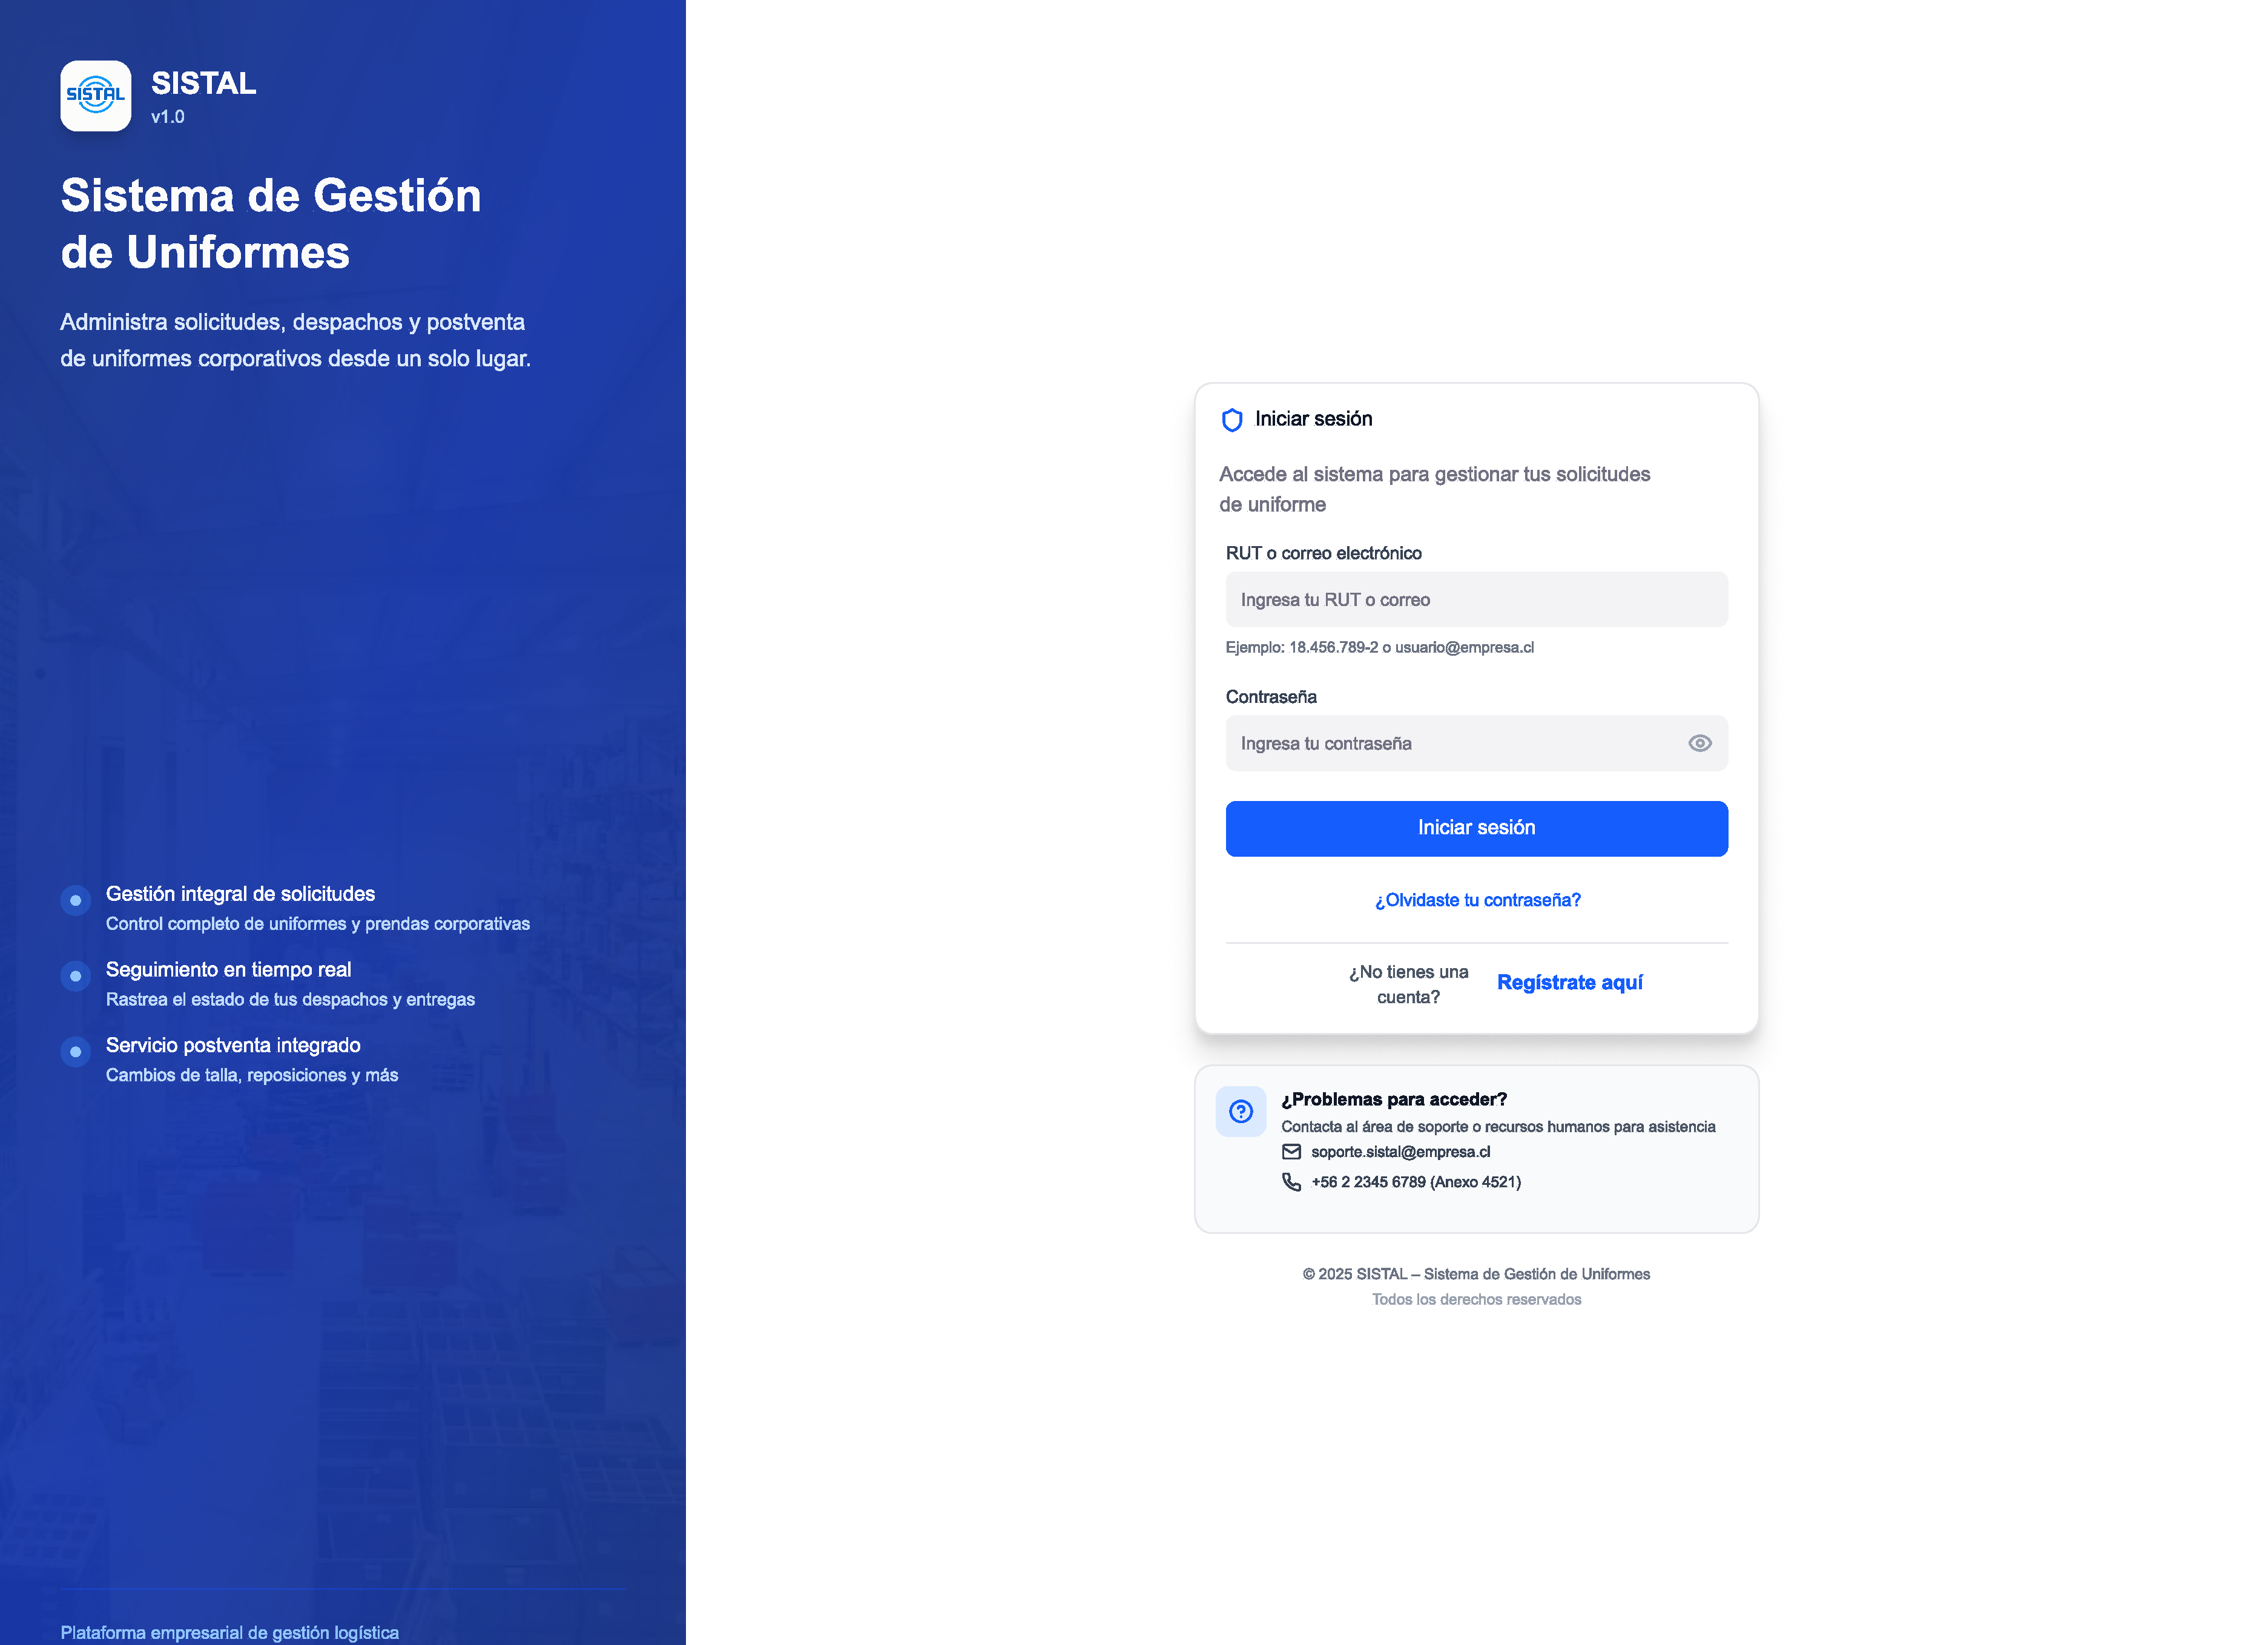
\includegraphics[width=0.9\textwidth, frame]{figuras/figma/Inicio de sesión.pdf}
    \caption{GUI de inicio de sesión} \label{fig:figma-login}
    \sourcefig{Elaboración Propia en Figma}{}{}
\end{sidewaysfigure}
\newpage

\begin{sidewaysfigure}
    \centering
    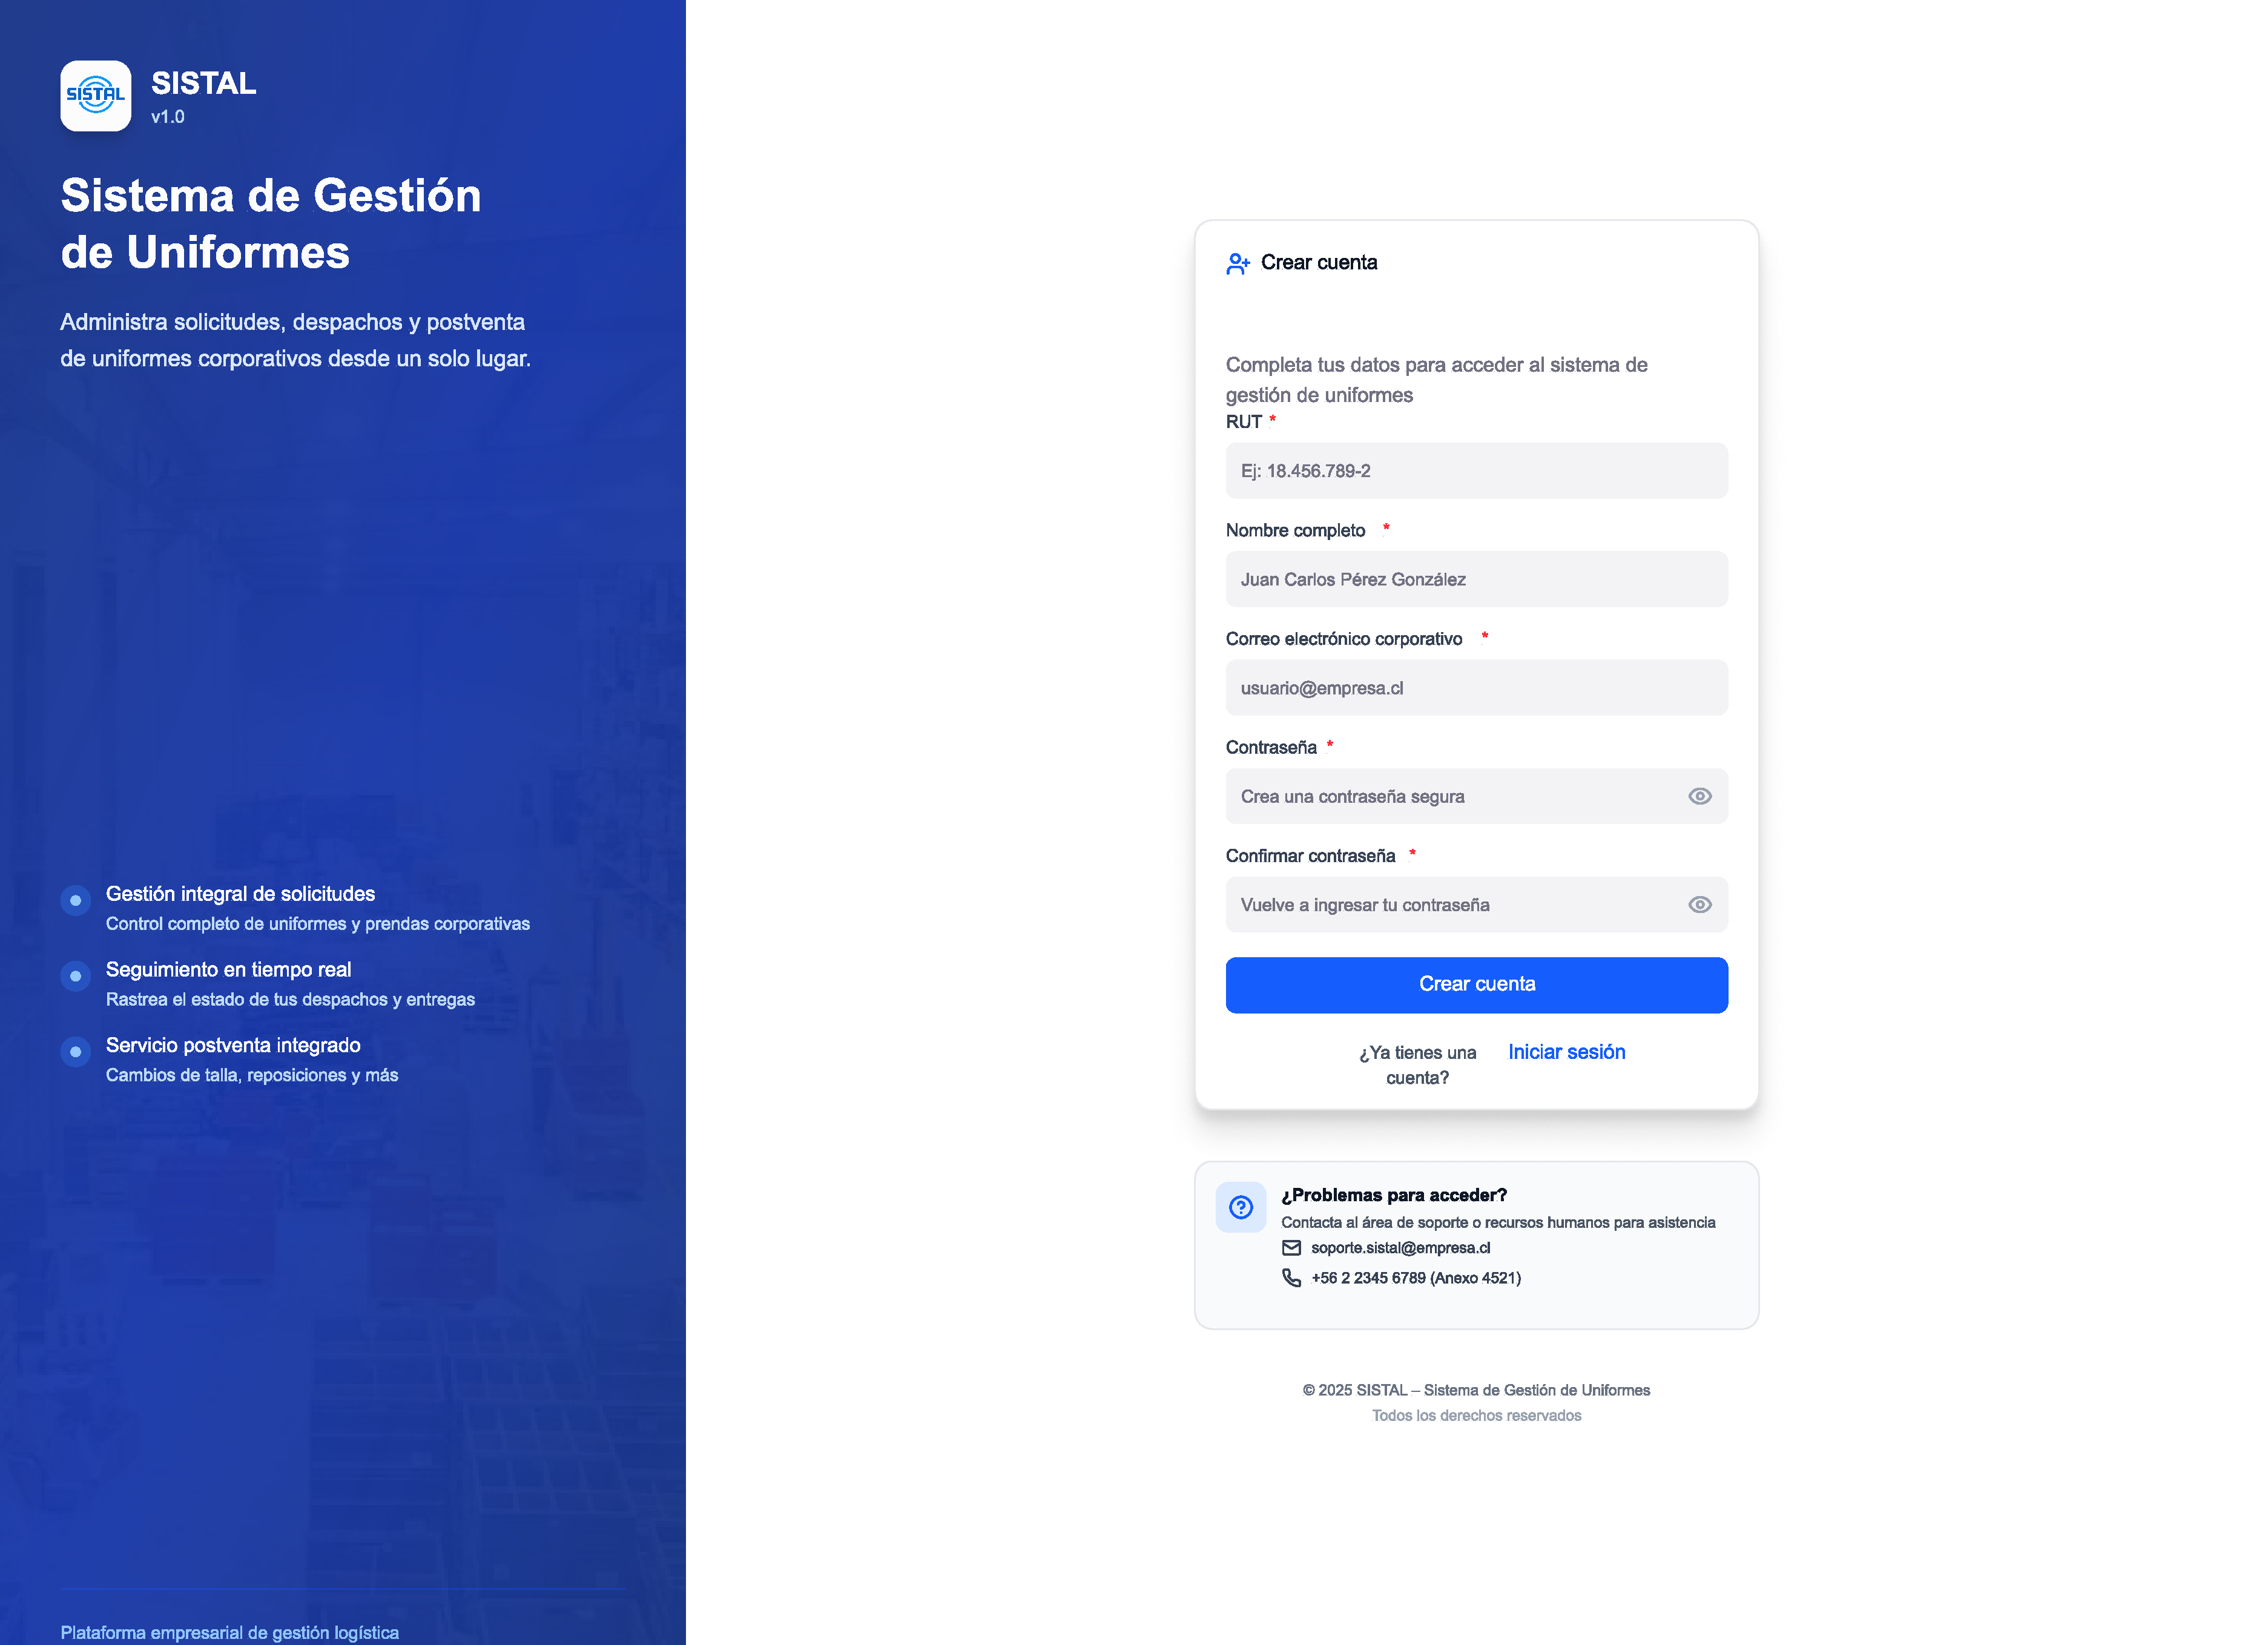
\includegraphics[width=0.9\textwidth, frame]{figuras/figma/Registro.pdf}
    \caption{GUI de registro de usuario} \label{fig:figma-registro}
    \sourcefig{Elaboración Propia en Figma}{}{}
\end{sidewaysfigure}
\newpage

\begin{figure}[p]
    \centering
    \includegraphics[width=\linewidth, frame]{figuras/figma/Wireframe Mis Solicitudes.pdf}
    \caption{GUI Panel principal de Funcionario} \label{fig:figma-funcionario}
    \sourcefig{Elaboración Propia en Figma}{}{}
\end{figure}

\begin{figure}[p]
    \centering
    \includegraphics[width=0.8\linewidth]{figuras/figma/Notificaciones.pdf}
    \caption{GUI Botón de notificaciones} \label{fig:figma-notificaciones}
    \sourcefig{Elaboración Propia en Figma}{}{}
\end{figure}

\begin{sidewaysfigure}
    \centering
    \includegraphics[width=\textheight, frame]{figuras/figma/Mis Solicitudes.pdf}
    \caption{GUI solicitudes realizadas por el funcionario} \label{fig:figma-solicitudes}
    \sourcefig{Elaboración Propia en Figma}{}{}
\end{sidewaysfigure}

\begin{figure}[p]
    \centering
    \includegraphics[height=0.93\textheight, frame]{figuras/figma/Solicitud cambio de sucursal.pdf}
    \caption{GUI de solicitud de cambio de sucursal} \label{fig:figma-cambio-sucursal}
    \sourcefig{Elaboración Propia en Figma}{}{}
\end{figure}

\begin{figure}[p]
    \centering
    \includegraphics[width=\linewidth, frame]{figuras/figma/Solicitud cambio de talla.pdf}
    \caption{GUI de solicitud de cambio de talla} \label{fig:figma-cambio-talla}
    \sourcefig{Elaboración Propia en Figma}{}{}
\end{figure}

\begin{sidewaysfigure}
    \centering
    \includegraphics[width=\textheight, frame]{figuras/figma/Seguimiento del despacho.pdf}
    \caption{GUI de seguimiento de despachos} \label{fig:figma-despachos}
    \sourcefig{Elaboración Propia en Figma}{}{}
\end{sidewaysfigure}

\begin{figure}[p]
    \centering
    \includegraphics[height=0.93\textheight, frame]{figuras/figma/Mi Cuenta.pdf}
    \caption{GUI de información de cuenta funcionario} \label{fig:figma-cuenta}
    \sourcefig{Elaboración Propia en Figma}{}{}
\end{figure}

    
    \chapter*{Conclusiones}
\addcontentsline{toc}{chapter}{CONCLUSIONES}



% -----------------------------------------------------------

El desarrollo del proyecto permitió comprobar que la reingeniería de un sistema monolítico, carente de estructura y buenas prácticas, puede abordarse de manera efectiva mediante una arquitectura moderna basada en servicios desacoplados, contenedores y despliegue en la nube. El proyecto demuestra que se puede migrar desde una solución obsoleta hacia una plataforma más mantenible, escalable y alineada con estándares actuales de la industria del software.

La posibilidad de mejorar la calidad estructural del sistema mediante la adopción de una arquitectura cloud-native y una pila tecnológica moderna, fue validada a través de la implementación funcional del módulo de funcionarios. Dicha implementación evidenció mejoras concretas en la separación de responsabilidades, integridad de los datos y automatización del ciclo de vida del software, además de lograr implementar un módulo completo en un corto periodo de tiempo.

En cuanto a los alcances del trabajo, se logró diseñar una arquitectura completa y desplegable, acompañada de un modelo de datos normalizado, flujos de integración y despliegue continuo, y una organización del desarrollo basada en buenas prácticas de control de versiones y gestión de tareas.

Desde el punto de vista disciplinar, el proyecto aporta un caso práctico de reingeniería de software aplicada, integrando arquitectura de microservicios, DevOps y computación en la nube, lo que resulta relevante tanto para contextos académicos como profesionales. La experiencia obtenida refuerza la importancia de abordar los problemas de sistemas heredados desde una perspectiva arquitectónica y no únicamente tecnológica.

Dentro de las dificultades presentadas en el proyecto, se encuentran el proceso inicial de familiarización del sistema, la cual consumió la mayor parte del tiempo y requirió de muchas reuniones. También nos encontramos con diversos desafíos tecnológicos ya que muchas de las tecnologías aplicadas en este proyecto no se abordan dentro del transcurso de la carrera.

% Las conclusiones pueden incluir los resultados obtenidos en la investigación, comprobación o refutación de la hipótesis, recomendaciones que puedan ser útiles al problema de investigación, reflejando a su vez los alcances y limitaciones del trabajo, aportes al campo o disciplina del conocimiento y conclusiones generales.
% 
% Deben tener una redacción clara, concreta y directa; no son un resumen de la investigación.


    % \include{cheatsheet}
    % ================ Bibliografía ====================

    \begingroup
        \linespread{2}
        \titlespacing*{name=\chapter,numberless}{0pt}{-39pt}{20pt}
        \printbibliography
        \addcontentsline{toc}{chapter}{BIBLIOGRAFÍA}
    \endgroup

    % ================ Glosario ========================

    \printglossary[type=negocio, title={Glosario del Negocio}]
    \addcontentsline{toc}{chapter}{GLOSARIO}
    \addcontentsline{toc}{section}{Glosario del Negocio}

    \printglossary[type=tech, title={Glosario Técnico}]
    \addcontentsline{toc}{section}{Glosario Técnico}

    \printglossary[type=acronym]
    \addcontentsline{toc}{section}{Siglas}

    % ================ Anexos ========================
    %\appendix
\addtocontents{toc}{\protect\renewcommand{\protect\cftchappresnum}{ANEXO~}}

\chapter{NUEVO DISEÑO DE INTERFAZ DE USUARIO}

\begin{sidewaysfigure}
    \centering
    \includegraphics[width=0.9\textwidth, frame]{figuras/figma/Inicio de sesión.pdf}
    \caption{GUI de inicio de sesión} \label{fig:figma-login}
    \sourcefig{Elaboración Propia en Figma}{}{}
\end{sidewaysfigure}
\newpage

\begin{sidewaysfigure}
    \centering
    \includegraphics[width=0.9\textwidth, frame]{figuras/figma/Registro.pdf}
    \caption{GUI de registro de usuario} \label{fig:figma-registro}
    \sourcefig{Elaboración Propia en Figma}{}{}
\end{sidewaysfigure}
\newpage

\begin{figure}[p]
    \centering
    \includegraphics[width=\linewidth, frame]{figuras/figma/Wireframe Mis Solicitudes.pdf}
    \caption{GUI Panel principal de Funcionario} \label{fig:figma-funcionario}
    \sourcefig{Elaboración Propia en Figma}{}{}
\end{figure}

\begin{figure}[p]
    \centering
    \includegraphics[width=0.8\linewidth]{figuras/figma/Notificaciones.pdf}
    \caption{GUI Botón de notificaciones} \label{fig:figma-notificaciones}
    \sourcefig{Elaboración Propia en Figma}{}{}
\end{figure}

\begin{sidewaysfigure}
    \centering
    \includegraphics[width=\textheight, frame]{figuras/figma/Mis Solicitudes.pdf}
    \caption{GUI solicitudes realizadas por el funcionario} \label{fig:figma-solicitudes}
    \sourcefig{Elaboración Propia en Figma}{}{}
\end{sidewaysfigure}

\begin{figure}[p]
    \centering
    \includegraphics[height=0.93\textheight, frame]{figuras/figma/Solicitud cambio de sucursal.pdf}
    \caption{GUI de solicitud de cambio de sucursal} \label{fig:figma-cambio-sucursal}
    \sourcefig{Elaboración Propia en Figma}{}{}
\end{figure}

\begin{figure}[p]
    \centering
    \includegraphics[width=\linewidth, frame]{figuras/figma/Solicitud cambio de talla.pdf}
    \caption{GUI de solicitud de cambio de talla} \label{fig:figma-cambio-talla}
    \sourcefig{Elaboración Propia en Figma}{}{}
\end{figure}

\begin{sidewaysfigure}
    \centering
    \includegraphics[width=\textheight, frame]{figuras/figma/Seguimiento del despacho.pdf}
    \caption{GUI de seguimiento de despachos} \label{fig:figma-despachos}
    \sourcefig{Elaboración Propia en Figma}{}{}
\end{sidewaysfigure}

\begin{figure}[p]
    \centering
    \includegraphics[height=0.93\textheight, frame]{figuras/figma/Mi Cuenta.pdf}
    \caption{GUI de información de cuenta funcionario} \label{fig:figma-cuenta}
    \sourcefig{Elaboración Propia en Figma}{}{}
\end{figure}


\end{document}
